% PLEASE USE THIS FILE AS A TEMPLATE
% Check file iosart2x.tex for more examples

\documentclass[ao]{iosart2x}
\usepackage{longtable}
\usepackage{lscape}
\usepackage{subcaption}

%%%%%%%%%%% Put your definitions here

\hypersetup{
pdfpagemode={UseOutlines},
bookmarksopen=true,
bookmarksopenlevel=1,
colorlinks=true,% Set to false to disable coloring links
citecolor=blue,% The color of citations
linkcolor=blue,% The color of references to document elements (sections, figures, etc)
urlcolor=blue,% The color of hyperlinks (URLs)
breaklinks=true,
}
% If you use the hyperref package, please uncomment the following line
% to display URLs in blue roman font according to Springer's eBook style:
\renewcommand\UrlFont{\color{blue}\rmfamily}

% this package need to be put after \usepackage[bookmarks=true]{hyperref} 
\usepackage{bookmark}


\usepackage{xcolor}
\definecolor{darkblue}{rgb}{0.0, 0.0, 0.55}
\definecolor{darkgreen}{rgb}{0.0, 0.2, 0.13}
\newcommand*{\q}[1]{\textcolor{red}{#1}}
\usepackage{listingsutf8} % for code snippets
\lstset{
    basicstyle=\ttfamily\scriptsize,
    columns=fullflexible,
    showstringspaces=false,
    numbers=none,
    numberstyle=\scriptsize,
    numbersep=5pt,
    extendedchars=true,
    literate={à}{{\`a}}1 {é}{{\'e}}1 {è}{{\`e}}1 {ê}{{\^e}}1 {ô}{{\^o}}1 {î}{{\^i}}1 {ï}{{\¨i}}1,
    inputencoding=utf8,
    breaklines=true,
    breakatwhitespace=false, % so url with no space will wrap
    postbreak=\mbox{\textcolor{brown}{$\hookrightarrow$}\space}
}

\lstdefinelanguage{turtle}
{
  morestring=[b][\color{darkgreen}]",
  morestring=[s][\color{darkblue}]{<}{>},
  moredelim=[s][\color{orange}]{\^{}}{\ },
  moredelim=[l][]{\:}{:},
  morecomment=[l][\color{gray}]{\#},
  identifierstyle=\color{black},
  keywords={@prefix,a},
  keywordstyle=\color{red},
  morekeywords=[2]{rdf,rdfs,xsd,foaf,dc,xml,owl,ex,cdt,qudt,unit,gr,cocoon,schema,ssn,sosa, prov, provone, weprov, data, dcterms},
  keywordstyle=[2]\color{cyan}
}

\lstset{language=turtle}

% Language Definitions for SPARQL
\lstdefinelanguage{sparql}{
morecomment=[l][\color{darkgreen}]{\#},
morestring=[b][\color{blue}]\",
morekeywords={SELECT,CONSTRUCT,DESCRIBE,ASK,WHERE,FROM,NAMED,PREFIX,BASE,OPTIONAL,FILTER,GRAPH,LIMIT,OFFSET,SERVICE,UNION,EXISTS,NOT,BINDINGS,MINUS,a,VALUES,AS,COUNT, GROUP, ORDER ,BY, EXIST, AS, MAX},
sensitive=true
}

%%%%%%%%%%% End of definitions

\pubyear{2020}
\volume{0}
\firstpage{1}
\lastpage{1}

\begin{document}

\begin{frontmatter}

%\pretitle{}
\title{WePROV: An Ontology for workflow evolution provenance analytics}
\runtitle{WePROV: An ontology for workflow evolution provenance analytics}
%\subtitle{}

% For one author:
%\author{\inits{N.}\fnms{Name1} \snm{Surname1}\ead[label=e1]{first@somewhere.com}}
%\address{Department first, \orgname{University or Company name},
%Abbreviate US states, \cny{Country}\printead[presep={\\}]{e1}}

% Two or more authors:

\author{\inits{A.}\fnms{Anila Sahar} \snm{Butt}\ead[label=e1]{anila.butt@csiro.au}%
\thanks{Corresponding author. \printead{e1}.}%\thanks{Do not use capitals for the author's surname.}
} and \author{\inits{P.}\fnms{Peter} \snm{Fitch}\ead[label=e2]{peter.fitch@csiro.au}}
\address{CSIRO \orgname{Land and Water}, \cny{Australia}. \printead[presep={\\}]{e1,e2}}



\begin{abstract}
Scientific workflow evolution provenance is essential for tracking, attributing and comparing the scientific research. 
The data models to capture the provenance, known as provenance models, have been of broad interest and studied in many fields, including the semantic Web. The provenance ontologies proposed by the semantic Web community for scientific workflows describe workflow specifications and their executions; however, they overlook workflow evolution provenance that is imperative for comprehensive provenance analytics in the context of the scientific workflow.
In this paper, we present a Workflow Evolution Provenance ontology (WePROV) that defines concepts, features, attributes, and relations to describe a workflow and its evolution process. To this, we discuss the underline provenance model and the design process of the proposed ontology.
Further, we define the functional requirements for a workflow evolution ontology and validate the proposed ontology through SPARQL queries for these requirements. We also present WePROV aligned dataset, built using open-source scientific workflows, to demonstrate the real-world applicability of the ontology. 
Our research shows that an ontology capable of describing the workflows and their evolutionary activities in a generic, machine-readable and interoperable format, enables automatic tracking of workflow changes and traversing between their different versions. 
\end{abstract}

\begin{keyword}
\kwd{Scientific Workflow}
\kwd{Workflow Evolution}
\kwd{Provenance Ontology}
\end{keyword}

\end{frontmatter}

%%%%%%%%%%% The article body starts:
\section{Introduction}

Scientific workflows are the popular mechanism for specifying and automating repetitive experiments~\citep{deelman2018future}. 
A significant aspect of their value lies in their potential to be reused. Once specified and shared, a workflow becomes a useful building block that can be combined or modified for developing new experiments~\citep{belhajjame2015using}. 
These workflows encapsulate a vast amount of knowledge associated with any scientific experiments~\citep{withana2010versioning}. 
When a workflow is used continuously over an extended period, the research is likely to evolve along different dimensions,
which causes the associated workflow to evolve. 
%Capturing the evolution of such workflows, known as their evolution provenance, is imperative for comprehensive provenance analytics in the context of the scientific workflows~\citep{anila_prov_2020}. 
Maintaining a detailed provenance of this process has many benefits that go beyond documentation and result in reproducibility~\citep{anila_prov_2020}. 
For example, this provenance information can be used to visualise the development of the research to see the path to the current state and what the previous attempts were. 
Also, some scientists may backtrack the workflow to a prior version and take a new direction. There might be an error in a model or an experiment, and this provenance can trace back the origin of that error. Alternatively, it helps to retrieve data products and results affected by this error. %Finally, in addition to tracing the workflows over time, scientists may also be interested in reproducing workflows~\citep{barga2010provenance}. 

Various Scientific Workflow Management Systems (SWfMSs) have been proposed and developed to provide an environment for specifying and enacting workflows (e.g., Taverna~\citep{hull2006taverna}, Kepler~\citep{altintas2004kepler}, Triana~\citep{taylor2007triana}, and YAWL~\citep{van2005yawl}). 
State-of-the-art SWfMSs automatically capture workflow provenance in the form of execution traces.
There also exist stand-alone approaches to capture and analyse the provenance of scientific workflows~\citep{oliveira2018provenance,prabhune2018p}. 
However, most of the systems and approaches do not capture provenance of revising a workflow definition (workflow evolution), rather account the scientist for managing the evolution of workflow through existing means for versioning files, such as filenames and folders, version control systems like git\footnote{\url{https://github.com/}}, or workflow sharing websites like myExperiment\footnote{\url{https://www.myexperiment.org/workflows}}.
Only a few SWfMSs (e.g., Kepler~\citep{altintas2004kepler} and VisTrails~\citep{freire2006managing}) proposed solutions to automatically capture the limited amount of workflow evolution provenance. But these solutions rely on proprietary formats that make it difficult to reuse these solutions.  
To overcome this limitation, there is a need for an ontology to comprehensively represent scientific workflows and their evolution in a generic, machine-readable, and workflow-engine independent format. In this format, they can be annotated, queried, and understood without relying on a language specific to a workflow-engine. 
%Scientific workflows and their versions should be published in a language that is independent of workflow management systems to increase their reuse across diverse projects and domains~\citep{5175816}. 

In recent years, the semantic Web community has proposed provenance models to describe scientific workflows and their execution traces in a generic, machine-readable and interoperable format.
In this regard, the Wf4Ever~\citep{belhajjame2015using} project addresses challenges related to generically described scientific experiments through the \textit{wfdesc}\footnote{\url{http://wf4ever.github.io/ro/\#wfdesc}} ontology, and an analysis and management of their execution provenance through the \textit{wfprov}\footnote{\url{http://wf4ever.github.io/ro/\#wfprov}} ontology.  
The Open Provenance Model for Workflows (OPMW)~\citep{Garijo:2011:NAP:2110497.2110504} presents a framework to publish computational workflows, which includes the specification of the \textit{OPMW}\footnote{\url{https://www.opmw.org/model/OPMW/}} ontology, for the description of workflow traces and their templates. 
ProvONE~\citep{cuevas2016provone} is another provenance model for scientific workflow, which is compatible with PROV-DM\footnote{\url{https://www.w3.org/TR/prov-dm/}} and provides constructs to model workflow specification and workflow execution provenance. 
All these models can capture, store, and query the provenance of workflows. However, they are unable to specify workflow evolution provenance. 

It is critical to understand the workflow evolution handling approach before designing an ontology for scientific workflows provenance. There are three main approaches to handle evolving workflows~\citep{kradolfer1999dynamic}. 
The first approach consists of allowing workflow modifications without retaining the pre-modification state. Each change is applied irreversibly to the workflow, considering possible consequences to the previous execution traces of this workflow. In this approach, tracking or reproducibility is not possible.
With the second approach, the state of workflow and its execution traces prior to the modifications are conserved. This approach allows tracking and traversing among versions; however, it requires managing a set of workflow versions. 
The third approach records only the latest workflow version and its difference (i.e., $\Delta$) from the previous version. This approach can reconstruct the previous versions, on-demand, without having to maintain a version database. %Considering this approach to be the one that allows tracking and traversing among its versions, without managing a set of workflow versions, we prefer the third approach.
This approach is concise and requires substantially less space than the alternative of storing multiple versions of a workflow specification~\citep{roddick1995survey}; therefore, we prefer this approach.

Based on above discussion, the main question to answer in this research is: \textbf{How can we design an ontology to enable automatic tracking of workflow changes and traversing between its different versions without recording a set of workflow versions?} 
To answer this question, we propose the Workflow Evolution Provenance ontology (WePROV) whose purpose is to identify and represent the fundamental concepts, attributes, and relations present in workflows and their evolution process. The ontology is built in a modular way to focus its reuse. As a part of the ontology design process, we first identify the functional requirements that an ontology must meet to be a comprehensive ontology for the workflow evolution provenance. Secondly, we explore the current ontologies to evaluate their reusability to design WePROV.  
Finally, we discuss three phases of the workflow lifecycle upon which we define four ontology design patterns to describe the workflow evolution provenance. Also, we present WePROV aligned dataset, built using open-source scientific workflows, to demonstrate the use of the ontology. 
Further, we validate the proposed ontology for its functional requirements through SPARQL queries. The evaluation shows that an ontology capable of describing the workflows and their evolutionary activities in a generic, machine-readable and interoperable format, enables automatic tracking of workflow changes and traversing between their different versions.

The rest of the paper is organised as follows. In Section~\ref{sec:motivation}, we motivate the need for workflow evolution provenance. In Section~\ref{sec:fundational_material}, we present the ontology development process. In Section~\ref{sec:weprov}, we discuss
the workflow evolution provenance ontology and the underline data model. In Section~\ref{sec:evaluation}, we evaluate our proposed ontology according to the community-defined best practices. In Section~\ref{sec:pre_work}, a review of the state-of-the-art is provided. Finally, we conclude our work in Section~\ref{sec:conclusion}.

\section{Motivation}
\label{sec:motivation}
The motives behind workflow evolution provenance stem from having to specify a workflow and reconsider the workflow structure and contents to satisfy the research or performance needs~\citep{koop2010provenance}. 
We identified three use cases that should be supported by an effective workflow evolution provenance system in close collaboration with SWfMS developers and experts. These experts are leading the development of the Senaps\footnote{\url{https://products.csiro.au/senaps/}} Platform and related projects. One of the expert, a team lead, worked very closely with the clients of the platform to understand the client's provenance needs. 
The three major use cases that motivated the need for a workflow evolution provenance system are:

\subsection{Tracking effects over time} 
When scientists associate their research with workflows, tracking the evolution of these workflows becomes an approximation to the initial problem of tracking the evolution of their research. Along with the evolution of a workflow, all its components evolve. Scientists should be able to look at the workflow evolution history and reason about how the research progressed at the current level to produce an output. 
Another critical aspect of tracking the evolution is to track the lineage and failure cause in the experiment. For example, 
if an algorithm or a workflow is erroneous, the evolution information helps to track the affected component or structure. %This information can be useful to revert to the last known right configuration and then start research from that point on-wards.

\subsection{Attribution} When a workflow is specified, attribution information such as who designed the experiment, who owns or created the workflow, who owns the data products can be gathered. This attribution information is useful to track down the issues or to give proper credit to the original owners. Also, while specifying workflows, it is becoming more common to reuse components (i.e., algorithms or models) within a workflow. Scientists utilise not only the algorithms and implementations developed by others but also the data products generated, including optimally derived model parameter configurations. For example, researchers within Digiscape\footnote{\url{https://research.csiro.au/digiscape/}} use the climate data published by the standard bodies to test their models. This reuse of a public corpus reduces effort and increases its acceptance. Tracking this kind of contribution not only provides a way to track contributions but also attribution for proper accreditation to the contributors. 

\subsection{Comparing Workflow Versions} A given research line might evolve in more than one direction. It is essential to understand the changes in these directions by comparing the difference between two or more versions of the same research. For example, given two outputs of two different versions of a workflow, one can deduce the reason for the difference between the two results by analysing the evolution information.

\section{Foundational Material}
\label{sec:fundational_material}
\subsection{Ontology Development Process}

The term ontology originates in philosophy. In computer science, there are several definitions of what an ontology is? We adopt the definition found in~\citep{studer1998knowledge}- \textit{``An ontology is a formal, explicit specification of a shared conceptualization''.} 
Ontology engineering is a complex process. %There are many methodologies found in the literature, e.g., the agile methodology RapidOWL~\citep{auer2006rapidowl}, Methontology~\citep{gomez1996towards}, and SABiO~\citep{de2014sabio,de1998systematic}. 
We followed a systematic approach presented in~\citep{de2014sabio} to build an ontology for evolution provenance of scientific workflows. This method considers activities for the development of reference ontologies and to its implementation as operational ontologies. %Also, we followed the FAIR principles\footnote{\url{https://www.force11.org/group/fairgroup/fairprinciples}} and the guidelines and best practices proposed by Noy and McGuinness.~\citep{noy2001ontology}.

\begin{figure}[h]
    \centering
    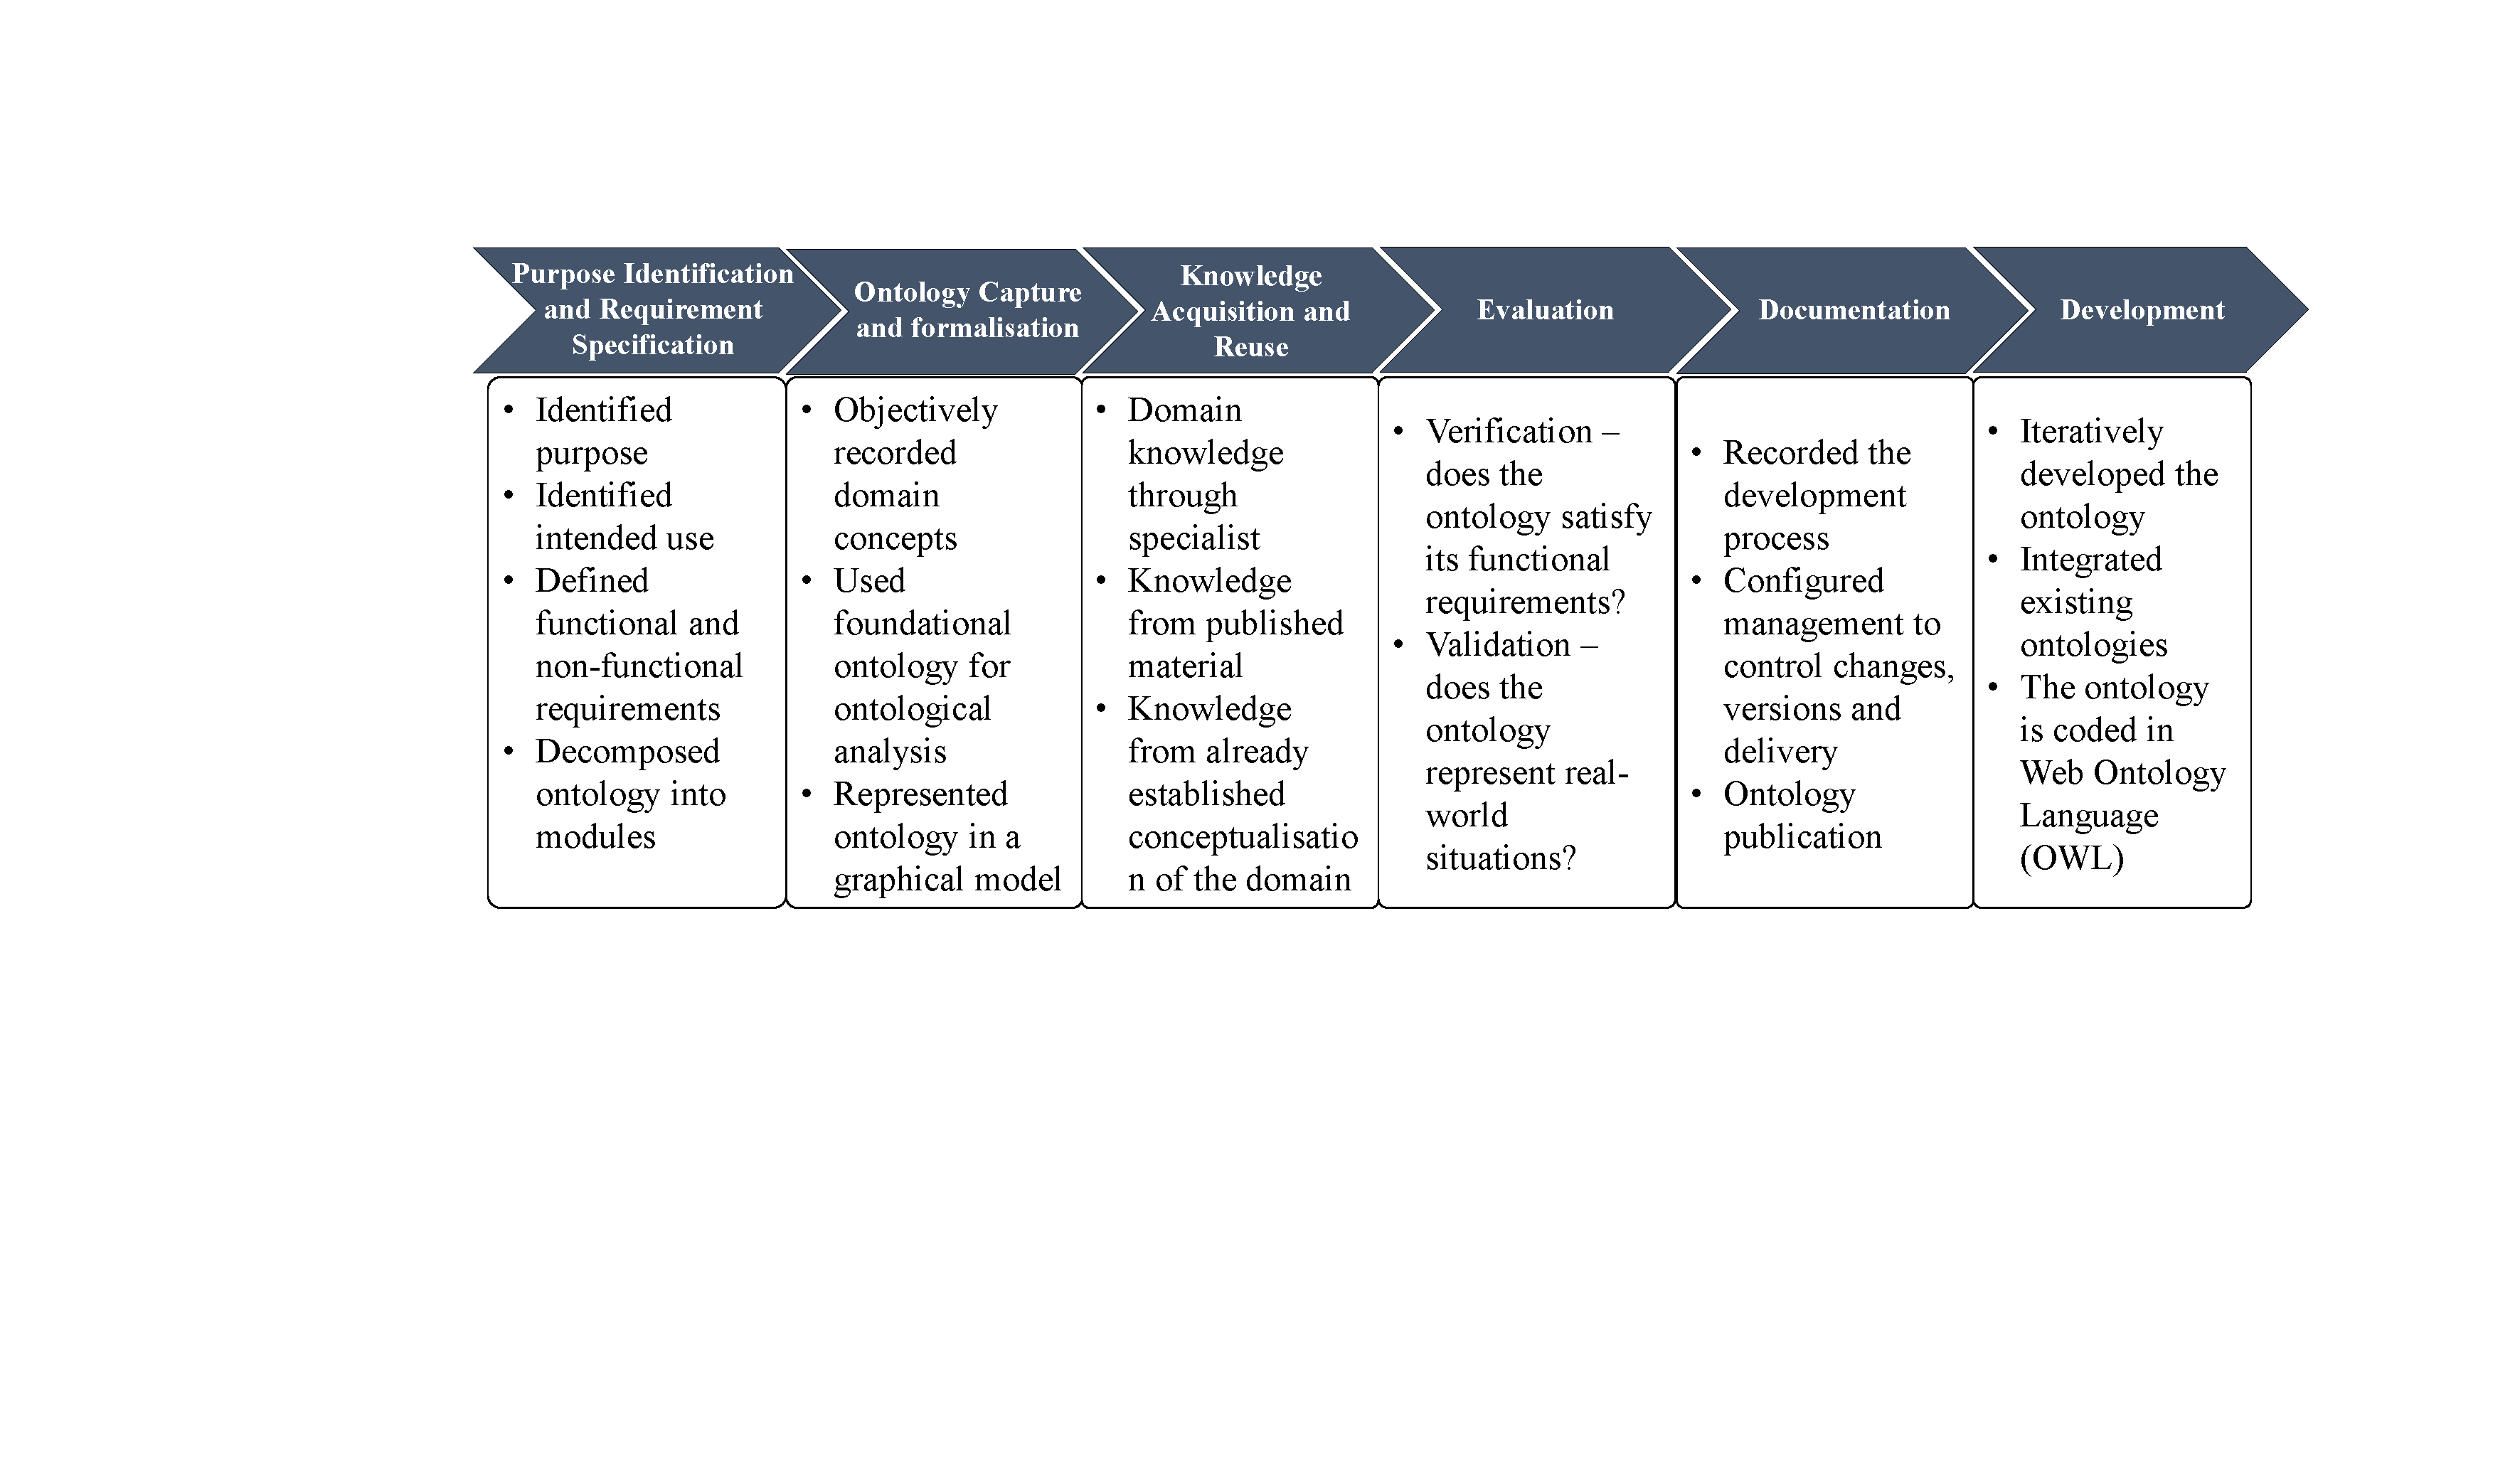
\includegraphics[width=\linewidth]{figures/ontology-development-process.pdf}
    \caption{Steps of the WePROV development process}
    \label{fig:development-process}
\end{figure}

The ontology development process includes six steps, as illustrated in Figure~\ref{fig:development-process}. 
In \textbf{Identification and Requirements Elicitation}, we identify the purpose and intended uses of the ontology, define its functional requirements through Competency Questions (CQs), and non-functional requirements (NFRs), and decompose the ontology into appropriate modules. 
During the \textbf{Ontology Capture and Formalisation} phase, we conceptualise the domain using a foundation ontology and represent it in a graphic model.
Also, for \textbf{Knowledge Acquisition}, we gather domain knowledge reliably through specialists and published material and take advantage of conceptualisations already established for the domain. 
For \textbf{Evaluation} purposes, we evaluate the suitability of the ontology through \textit{verification}, ensuring that the ontology satisfies its requirements, and \textit{validation}, ensuring that the ontology can represent real-world situations.
Further, the \textbf{Documentation} stage records the results of the development process using a Reference Ontology Specification followed by configuration management, which is performed through a repository to control changes, versions, and delivery. 
Ontology \textbf{Development} is an iterative process where each version is evaluated over the generic and domain-specific competency questions and iteratively improved by assessing its ability to answer the competency questions. After designing the ontology, we create instance repositories for workflow evolutions provenance and can answer the competency questions via SPARQL queries.

\subsection{Ontology Requirement Specification}
We closely collaborated with the developers of scientific workflow engines that includes WorkSpace \citep{cleary2015using,bolger2016workspace} and Senaps\footnote{\url{https://products.csiro.au/senaps/}} and provenance researchers from the CSIRO\footnote{\url{https://www.csiro.au/}}, the Australian National University\footnote{\url{https://www.anu.edu.au/}}, and SurroundAustralia\footnote{\url{https://surroundaustralia.com/}} to elicit the following functional and non-functional requirements for the WePROV ontology. 

\subsubsection{Non-functional Requirements}

We identified the following non-functional requirements: 

\begin{enumerate}
    \item[-]\textbf{NFR1:} Be modular or embedded in a modular framework to facilitate reuse of other ontologies and, consequently, its reuse by other ontologies.
    \item[-]\textbf{NFR2:} Be based on well-known sources from the literature. 
    \item[-]\textbf{NFR3:} Be documented in a standard-compliant and machine-readable format.
\end{enumerate}
 To address \textbf{NFR1}, we decompose the ontology into two modules namely, WePROV-workflow and WePROV-evolution. The former defines the components and structure of a workflow (Section~\ref{subsec:weprov-worflow}), and the latter defines the the main concepts and relationships to describe workflow evolution process (Section~\ref{subsec:weprov-evolution}).
 % The form provides an overview of the main concepts and relationships to describe workflow evolution, and the later defines a workflow and its elements. 
 As part of NFR1, we integrated WePROV into the Provenance Ontology (PROV-O) and the ProvONE ontology. The prefixes of these reused ontologies in WePROV are preceded by the corresponding acronyms (prov: and provone: respectively), throughout the paper. %and highlighted using different colours. 
Regarding \textbf{NFR2}, ontology capture is supported by the process of knowledge acquisition that used consolidated sources of knowledge referring to the scientific workflows in this research, including books and standards. Regarding \textbf{NFR3}, ontology is documented in a machine-readable format i.e., RDF/OWL.

\subsubsection{Functional Requirements}
\label{subsubsection:CQ}
The authors of this paper worked with Senaps team for more than twelve months to identified a series of tasks that need to be supported by a useful workflow evolution provenance ontology as the functional requirements. Next, the competency questions (CQs) are defined iteratively based on the identified tasks. %We have defined several relevant CQs detailed in WePROV's Reference Ontology Specification document [Reference]. 
Here, we list eleven of the most important CQs to evaluate the proposed ontology.
\begin{enumerate}
    \item[-]\textbf{CQ1:} \textbf{Find the temporal reconstruction of the workflow design.} Users want to understand the evolution of the research (i.e., workflow) since inception to date. The ontology should be able to provide information about different versions of the workflow, how often the workflow has evolved and at what point on time. An indication of the exact changes is also desirable. 
    \item[-]\textbf{CQ2:} \textbf{Identify different changes in a version of the workflow.} Users require to know if the contents or structures of the workflow have evolved to understand the rationale behind the changes. The ontology should support queries to identify all changes. 
%    \item[-]\textbf{CQ3:} \textbf{Identify different dimensions that have evolved for the workflow.} Users often require exploring those versions of workflows, which do not have sub-versions. An ontology that answers this question serves to understand all possible investigated dimensions explored to design the current version of the workflow.
    \item[-]\textbf{CQ3:} \textbf{Report the reason(s) of divergent results of two executions of a workflow.} Users are curious to identify the root cause of the unexpected behaviour of the workflow. One such reason could be the change in workflow, or it could be some accidental changes in the workflow. Comparing two versions pinpoint the changed composition of the workflow.
    \item[-]\textbf{CQ4:} \textbf{Which one is the most unstable component of the workflow?} Users are interested to know a component that is the reason of frequent changes in the workflow. The ontology should support the identification of the component that has frequent revisions.
    \item[-]\textbf{CQ5:} \textbf{Identify all the agents who have participated in the design of the workflow.} The ontology should be able to identify all participants who contributed to any version of the workflow instead of those who contributed to the latest/last version.
    \item[-]\textbf{CQ6:} \textbf{Who is responsible for a change in the workflow?} Users need to know who is responsible for a change in the workflow. This requirement is a typical auditing question that assigns responsibility to a participant for the change made.
    \item[-]\textbf{CQ7:} \textbf{Who participated in a specific (first/latest) version of the workflow?} Users need to attribute the work to an agent. This attribution information is useful to track down the issues or to give proper credit to the original participants. 
    \item[-]\textbf{CQ8:} \textbf{Find all workflows (or versions of a workflow) where an agent has participated.}  This question addresses the need to identify the work/research of an agent and its participation.  The ontology should support queries to find workflows, versions, and components where an agent has participated along with the time of participation.   
    \item[-]\textbf{CQ9:} \textbf{Find the collaborative researchers and their collaboration count of designing workflows together.} Users need to know researchers (i.e., agents) who most often collaborate and their count of collaborative workflows. This information could help in identifying collaborative communities who have similar research interests. 
    \item[-]\textbf{CQ10: When a (first/last) version of the workflow is created?}  Users need to know when the workflow was designed and since when it has not changed.  The ontology should be able to record the effect of time on workflow lifespan.
    \item[-]\textbf{CQ11: How long did an agent participate in a workflow (or repository of a workflow)?} Users need to identify the period a specific agent was active in the lifespan of a workflow. The ontology should answer the start and end time of an agent's participation. 
\end{enumerate}

\subsection{Knowledge Acquisition and Reuse}
It is crucial to understand the existing provenance ontologies for their reuse to design a workflow evolution provenance ontology. 
First, we consider PROV-DM, a conceptual data model that forms a basis for the W3C provenance ontology PROV-O in Section~\ref{subsec:prov-dm}. 
Next, we revisit some existing workflow provenance ontologies and evaluate their reusability to capture workflow evolution provenance in Section~\ref{subsec:workflow-specification-pattern}.

\subsubsection{PROV-DM: Baseline provenance model}
\label{subsec:prov-dm}

PROV provides a generic data model, PROV-DM\footnote{\url{https://www.w3.org/TR/prov-dm/}}, to outline the provenance.
It is a W3C recommendation and designed to be an agnostic model for provenance description from different areas. 
%Its data model can represent data transformations and ownership. PROV may be extended to fulfil the requirements of domains.
The PROV data model can represent data transformations and ownership, and it can be extended to fulfil the requirements of domains.
The classes \textit{Entity}, \textit{Activity}, and \textit{Agent} along with the relationships \textit{Used}, \textit{WasGeneratedBy}, \textit{WasInformedBy}, \textit{WasAssociatedWith}, \textit{WasDerivedFrom},
\textit{WasAttributedTo}, and \textit{ActedOnBehalfOf} form the core model of PROV-DM as shown in Figure~\ref{fig:prov-dm}.
The second component of PROV-DM is dealing with derivations of entities from other entities and derivation subtypes \textit{Revision}, \textit{Quotation}, and \textit{Primary Source}. 

\begin{figure}[h]
    \centering
    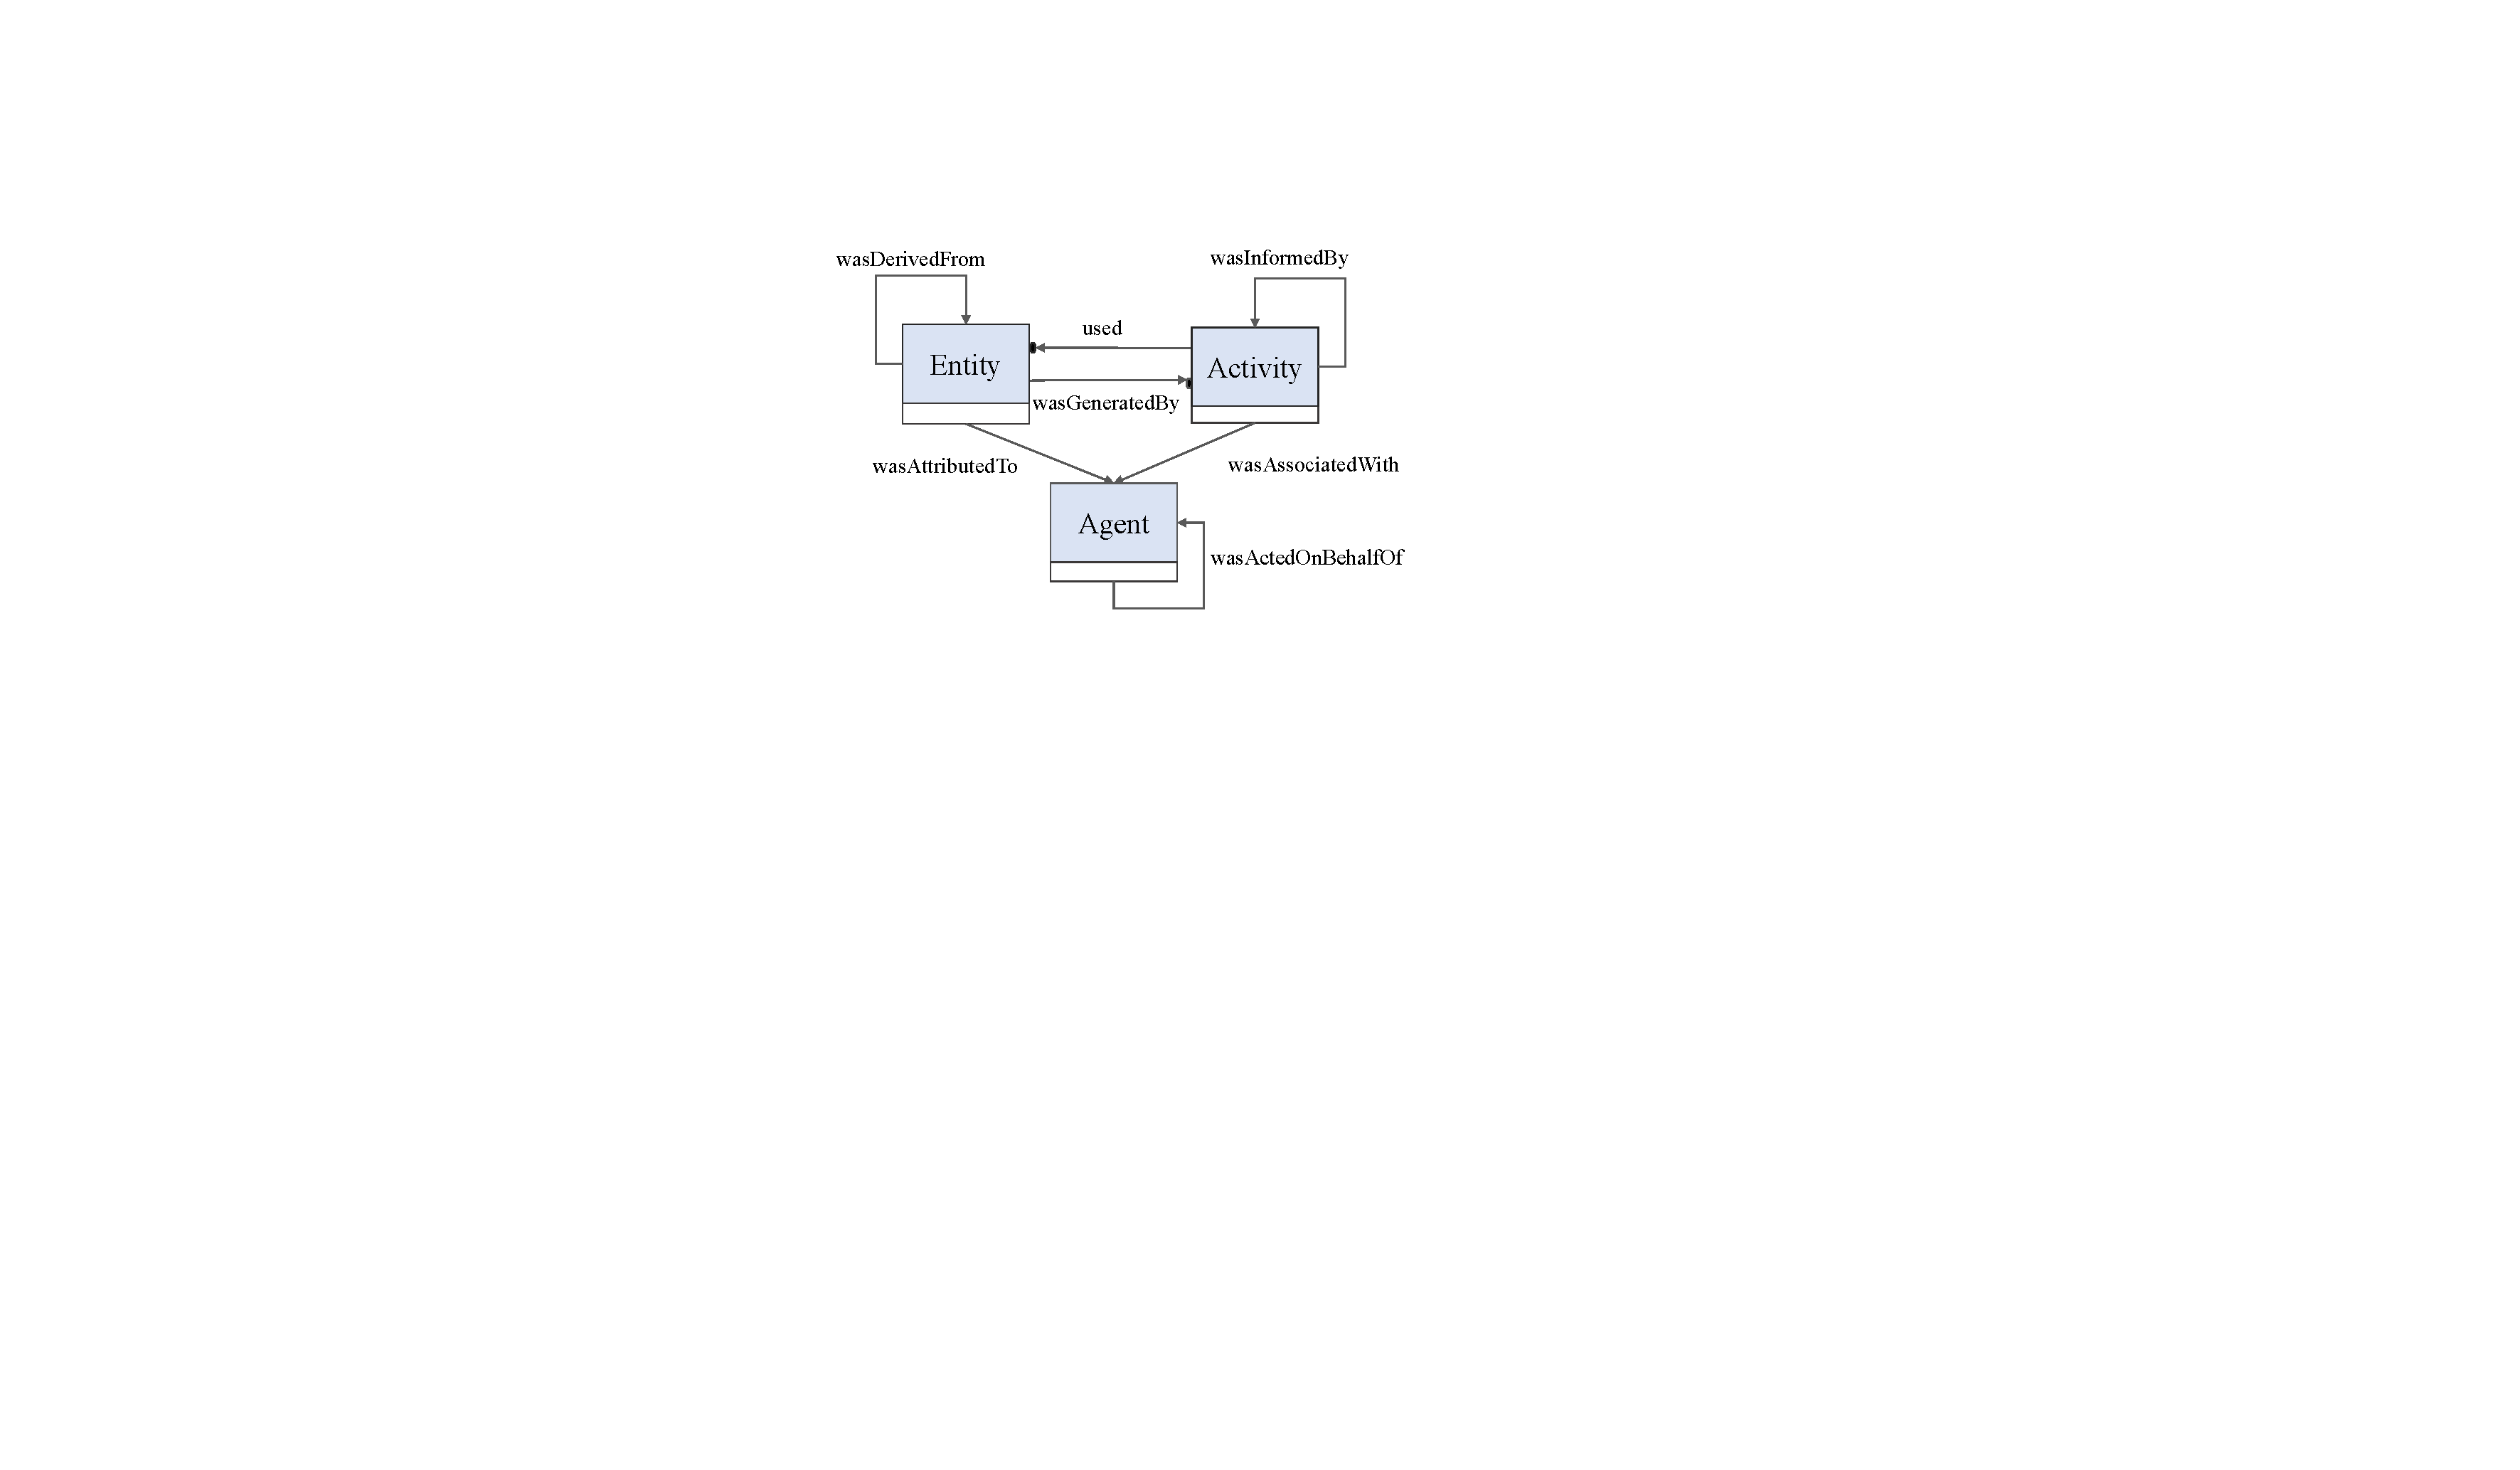
\includegraphics[width=0.5\linewidth]{figures/prov-o.pdf}
    \caption{PROV Core Structure}
    \label{fig:prov-dm}
\end{figure}

PROV is developed to promote an interoperable interchange of provenance in heterogeneous environments, such as the Web. However, it is a generic and domain-independent ontology, as it does not cater to the requirements of specific systems or domain applications. Instead, it provides extension points through which such systems and applications can extend PROV for their domain. Moreover, it is quite easy to come up with anyone’s own provenance ontology for a domain. However, the heterogeneous models to capture provenance of a domain of interest defeat the entire purpose of a community effort and thus breaks the interoperability, which is the central premise of PROV. Therefore, a standard provenance ontology is necessary for a domain to meet the interoperability goal of the Web. 

\subsubsection{Scientific workflow model}
\label{subsec:workflow-specification-pattern}

In recent years, the Semantic Web community has proposed provenance ontologies to formalise and describe scientific workflows and their execution traces and has shown several applications of these ontologies~\citep{oliveira2018provenance}. 
In this regard, Wf4Ever~\citep{belhajjame2015using}
project addresses challenges related to generically describing scientific experiments through the \textit{wfdesc} ontology, and an analysis and management of their execution provenance through the \textit{wfprov} ontology.  
The Open Provenance Model for Workflows (OPMW)~\citep{Garijo:2011:NAP:2110497.2110504} presents a framework to publish computational workflows including the specification of the \textit{OPMW} ontology, for the description of workflow traces and their templates.
As part of this framework, the authors also published the Ontology for Provenance and Plans (P-Plan)\footnote{\url{http://www.opmw.org/model/p-plan/}}. P-Plan extends the Provenance Ontology (PROV-O)~\citep{moreau2013PROV} to specify the plans that guide the execution of scientific processes, describing how such plans are composed and their correspondence to provenance records that describe the execution.
ProvONE~\citep{cuevas2016provone} is another provenance ontology to describe scientific workflow, which is compatible with PROV-DM. It provides constructs to describe workflow specification and workflow execution provenance. 
%All these ontologies are potential candidate of provenance ontology to capture, store, and query the provenance of workflows and their traces in a format, which is common, machine-readable, and independent of workflow-engine. 
Each of these ontologies can capture, store, and query the provenance of workflows and their traces in a common, machine-readable, and workflow-engine independent format.
However, they are unable to describe workflow evolution provenance. 
ProvONE supports a minimal level of evolution provenance. For instance, for a workflow shown in Figures~\ref{fig:v1} and~\ref{fig:v2}, Listing~\ref{lst:provone-prov} represents ProvONE aligned evolution provenance. 

\begin{figure}[htpb]
    \begin{minipage}{.45\textwidth}
        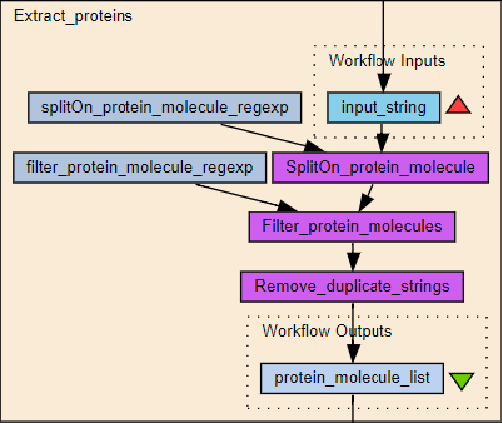
\includegraphics[width=0.95\linewidth]{figures/workflow-v0.pdf}
        \caption{Extract\_Proteins\_v1}
        \label{fig:v1}
    \end{minipage}
    \begin{minipage}{.45\textwidth}
        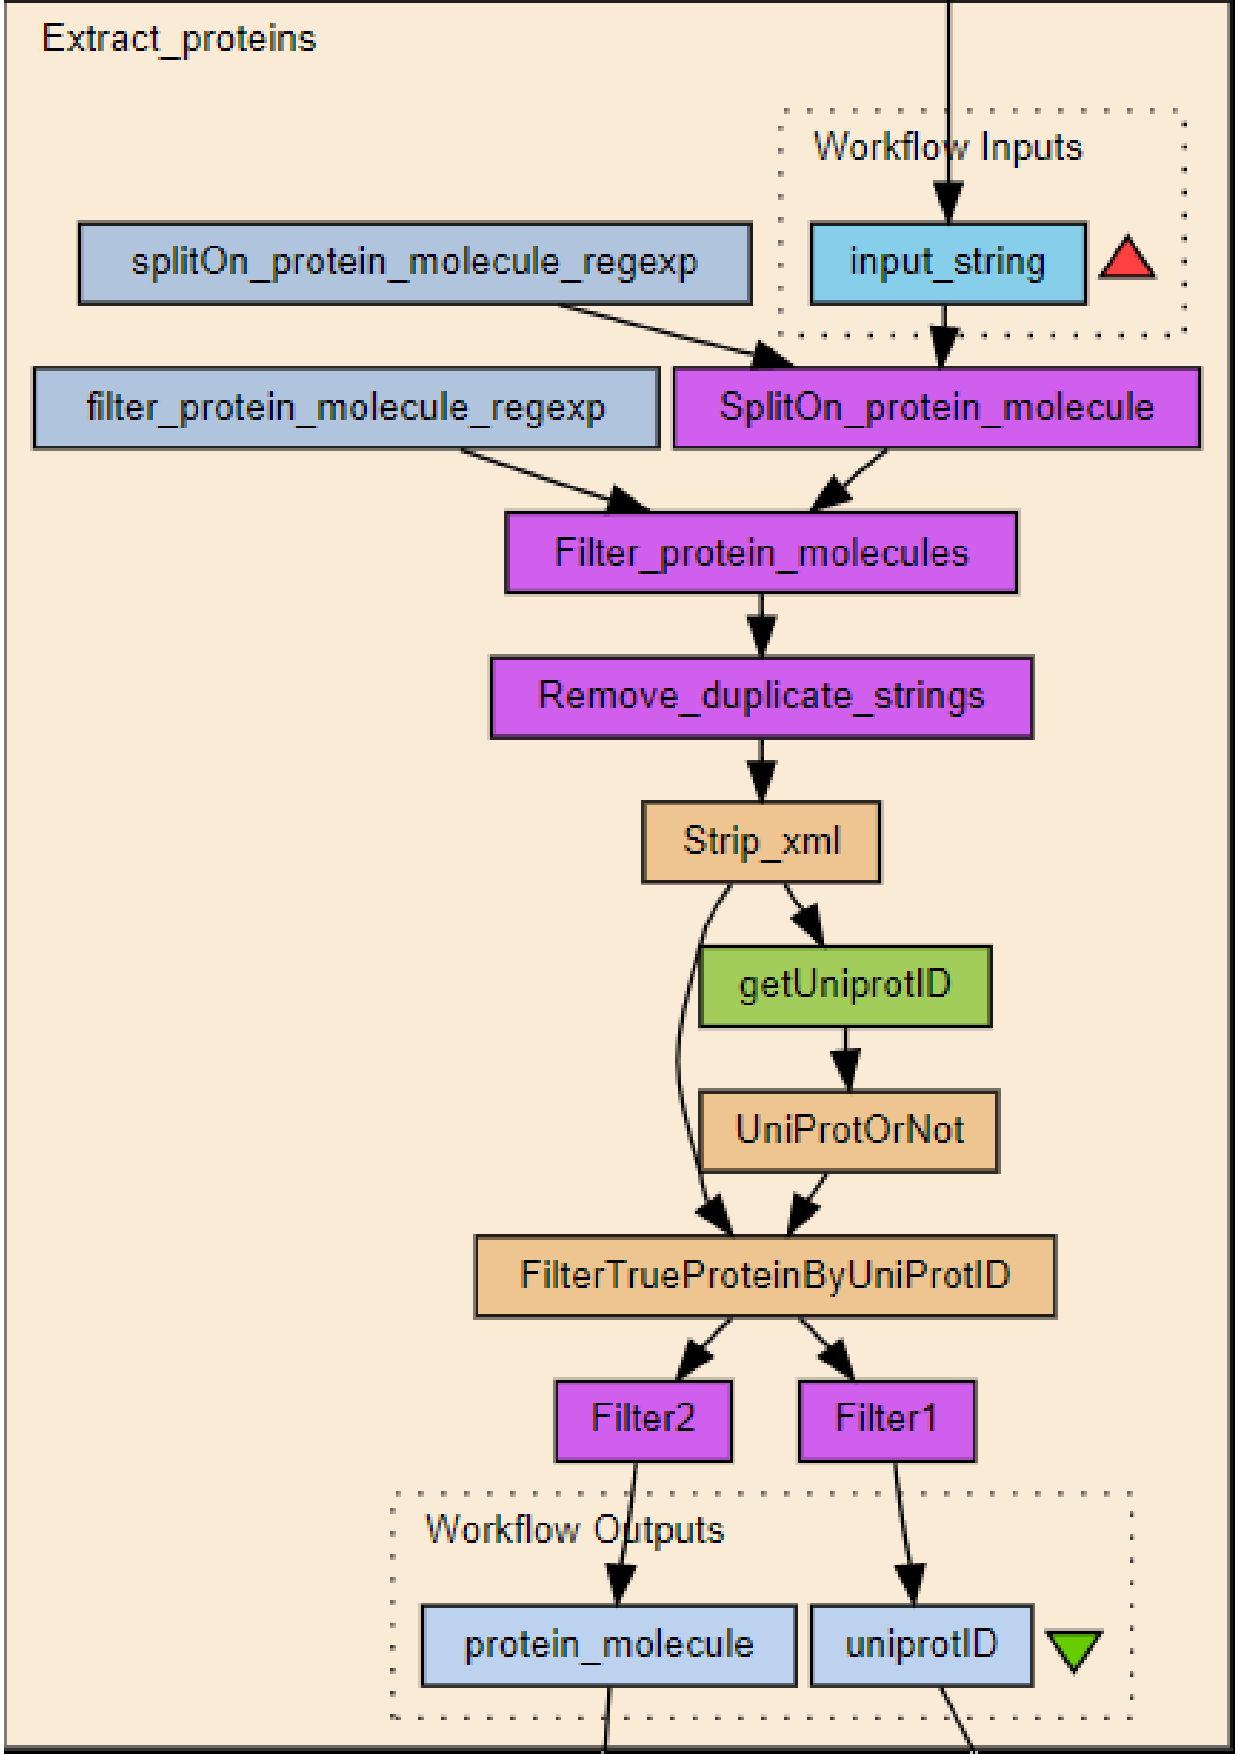
\includegraphics[width=0.95\linewidth]{figures/workflow-v1.pdf}
        \caption{Extract\_Proteins\_v2}
        \label{fig:v2}
    \end{minipage}
\end{figure}

Here, the versions of a workflow form a derivation tree, which is represented with \textit{wasDerivedFrom} association from PROV-O ontology. The evolution provenance captures that "Extract\_Proteins\_v2" is derived from "Extract\_Proteins\_v1". 
However, the specific changes performed in the specification of a workflow are uncaptured in ProvONE aligned evolution provenance. 

\begin{lstlisting}[frame=single, caption={ProvONE aligned evolution provenance},label={lst:provone-prov}]
@prefix rdfs:    <http://www.w3.org/2000/01/rdf-schema#> .
@prefix xsd:     <http://www.w3.org/2001/XMLSchema#> .
@prefix dcterms: <http://purl.org/dc/terms/> .
@prefix prov:    <http://www.w3.org/ns/prov#> .
@prefix provone: <http://purl.org/provone> .
@prefix :        <http://example.com/> .

:Extract_Proteins_v2
        rdf:type       provone:Workflow;
        dcterms:identifier "v2"^^xsd:string;
        dcterms:title "Extract_Proteins"^^xsd:string;
        
:Extract_Proteins_v2  prov:wasDerivedFrom   :Extract_Proteins_v1

\end{lstlisting}

In Section~\ref{sec:weprov}, we will provide a different perspective of evolution provenance, which \textit{wasDerivedFrom} association cannot capture. 

\section{WePROV: Workflow Evolution Provenance Modelling}
\label{sec:weprov}

To fulfil the need for workflow evolution provenance, we propose a \textbf{WePROV} - \textbf{W}orkflow \textbf{e}volution \textbf{PROV}enance ontology in this paper. 

\subsection{WePROV-Workflow}
\label{subsec:weprov-worflow}

In this regard, we need to formalise the structure and components of a workflow that can evolve and understand the provenance ontologies mentioned above for their reusability. ProvONE is a widely used workflow provenance ontology because of its ability to capture comprehensive scientific workflows provenance~\citep{prabhune2018p}. We reuse workflow specification pattern shown in Figure~\ref{fig:workflow-specification} from ProvONE and provide an additional layer to capture workflow evolution provenance.  

\begin{figure}[h]
    \centering
    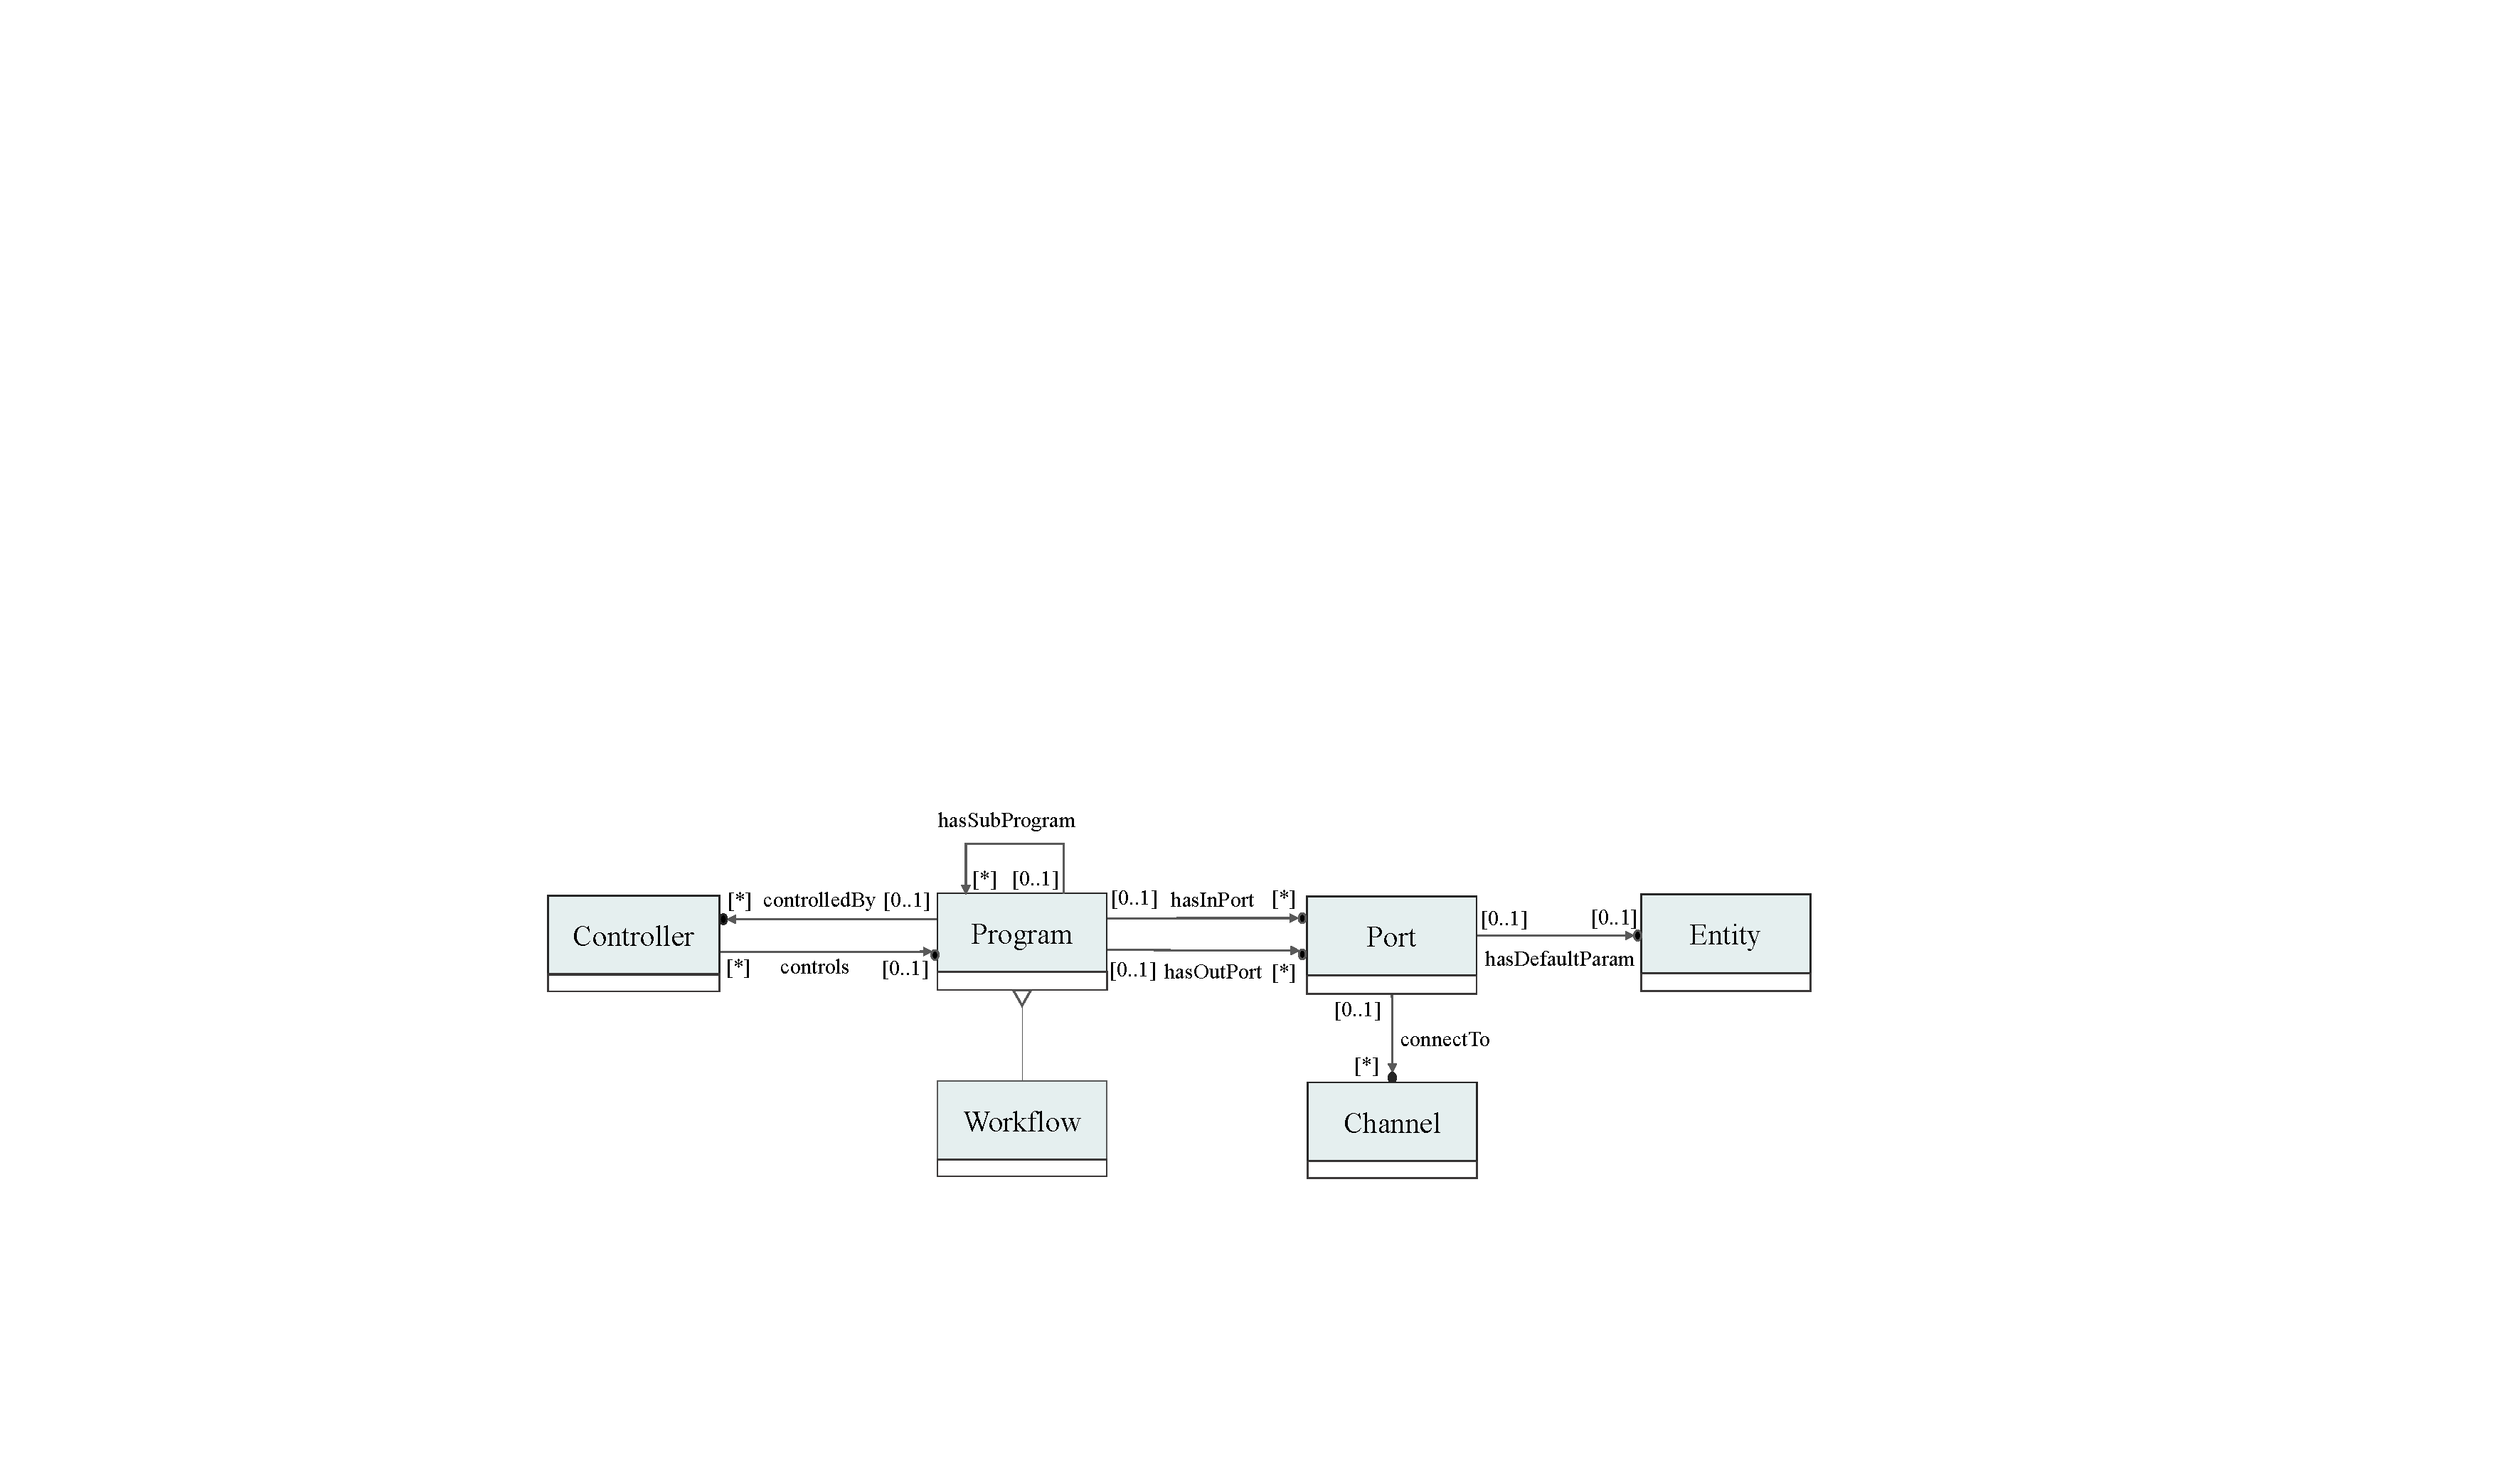
\includegraphics[width=0.9\linewidth]{figures/workflow-specs.pdf}
    \caption{Scientific Workflow Specification Model}
    \label{fig:workflow-specification}
\end{figure}

Figure~\ref{fig:workflow-specification} highlights the key components of a workflow, which can evolve and to which evolution provenance applies. 
\begin{itemize}
\item[-]\textbf{Program (\begin{math}\mathcal{P}\end{math}):} The various tasks that are part of a workflow are represented by the Program class. Programs can either be atomic or composite, the latter case specified through the \textit{hasSubProgram} self-association. A workflow itself is a program.

\item[-]\textbf{Port:} Each Program may have a series of Ports that function as input (\begin{math}\mathcal{I}\end{math}) or output (\begin{math}\mathcal{O}\end{math}) ports.

\item[-]\textbf{Channel (\begin{math}\mathcal{C}\end{math}):} Ports of the Programs connect through Channels. Both input and output ports may associate with multiple Channels. Connecting a single port to multiple channels capture workflows where a single output is copied and sent to multiple destinations. Moreover, it models workflows where tasks take inputs from different sources through a single input port.

\item[-] \textbf{Parameter  (\begin{math}\mathcal{A}\end{math}):} In order to specify executable instances of a Workflow, default parameters can be defined for some of its constituent programs. The default parameters are represented by Entities.

\item[-] \textbf{Controller (\begin{math}\mathcal{L}\end{math}):} A Controller class can be used to specify that the execution of a given program is controlled by another program, which allows for differing model of executions. For instance, in the asynchronous data flow model, a given Program may only start once the execution of a preceding program terminates.
\end{itemize} 

Based on the elements of a workflow, we defined our workflow as: 

\newtheorem{definition}{Definition}[section]
\begin{definition}\label{def:workflow}
A workflow \begin{math}\mathcal{W}\end{math} is a graph that connects programs \begin{math}\mathcal{P}\end{math} to data \begin{math}\mathcal{D}\end{math} and other programs in the graph through edges \begin{math}\mathcal{E}\end{math}.
\end{definition}
    \begin{equation}
            \mathcal{W} = (\mathcal{P}, \mathcal{D}, \mathcal{E})
    \end{equation}

    Where (\begin{math}\mathcal{I}\end{math} $\cup$ \begin{math}\mathcal{O}\end{math} $\cup$ \begin{math}\mathcal{A}\end{math}) $\in$ \begin{math}\mathcal{D}\end{math}  and (\begin{math}\mathcal{L}\end{math} $\cup$ \begin{math}\mathcal{C}\end{math}) $\in$ \begin{math}\mathcal{E}\end{math} 

\subsection{WePROV-Evolution}
\label{subsec:weprov-evolution}

Three phases of workflow evolution are considered within our approach: workflow creation, workflow deletion, and workflow modification, as shown in Figure~\ref{fig:workflow-evolution}. 
%Workflow creation (or deletion) considers the creation (or deletion) of a workflow and (or) its component. Workflow modification refers to the workflow update.
Workflow creation deals with two main activities that are related and, in some cases, overlap but are fundamentally different activities. A workflow can be created by creating new models and specifying a new workflow structure, or by merging and reusing existing workflows. The former is referred to workflow creation and the latter is referred to workflow derivation in this paper.
In Definition~\ref{def:workflow}, we defined a workflow with a graph in which nodes and edges correspond to operational tasks, and data flows between these tasks respectively. Therefore, two types of modification activities that affect the workflow are distinguished: structural modification (addition or deletion of nodes or edges); and content modification (modification of a node or an edge).
Sections~\ref{subsec:workflow-creation},~\ref{subsec:workflow-deletion}~and~\ref{subsec:workflow-modification} provide a detailed discussion on workflow evolution. 

\begin{figure}[htpb]
    \centering
    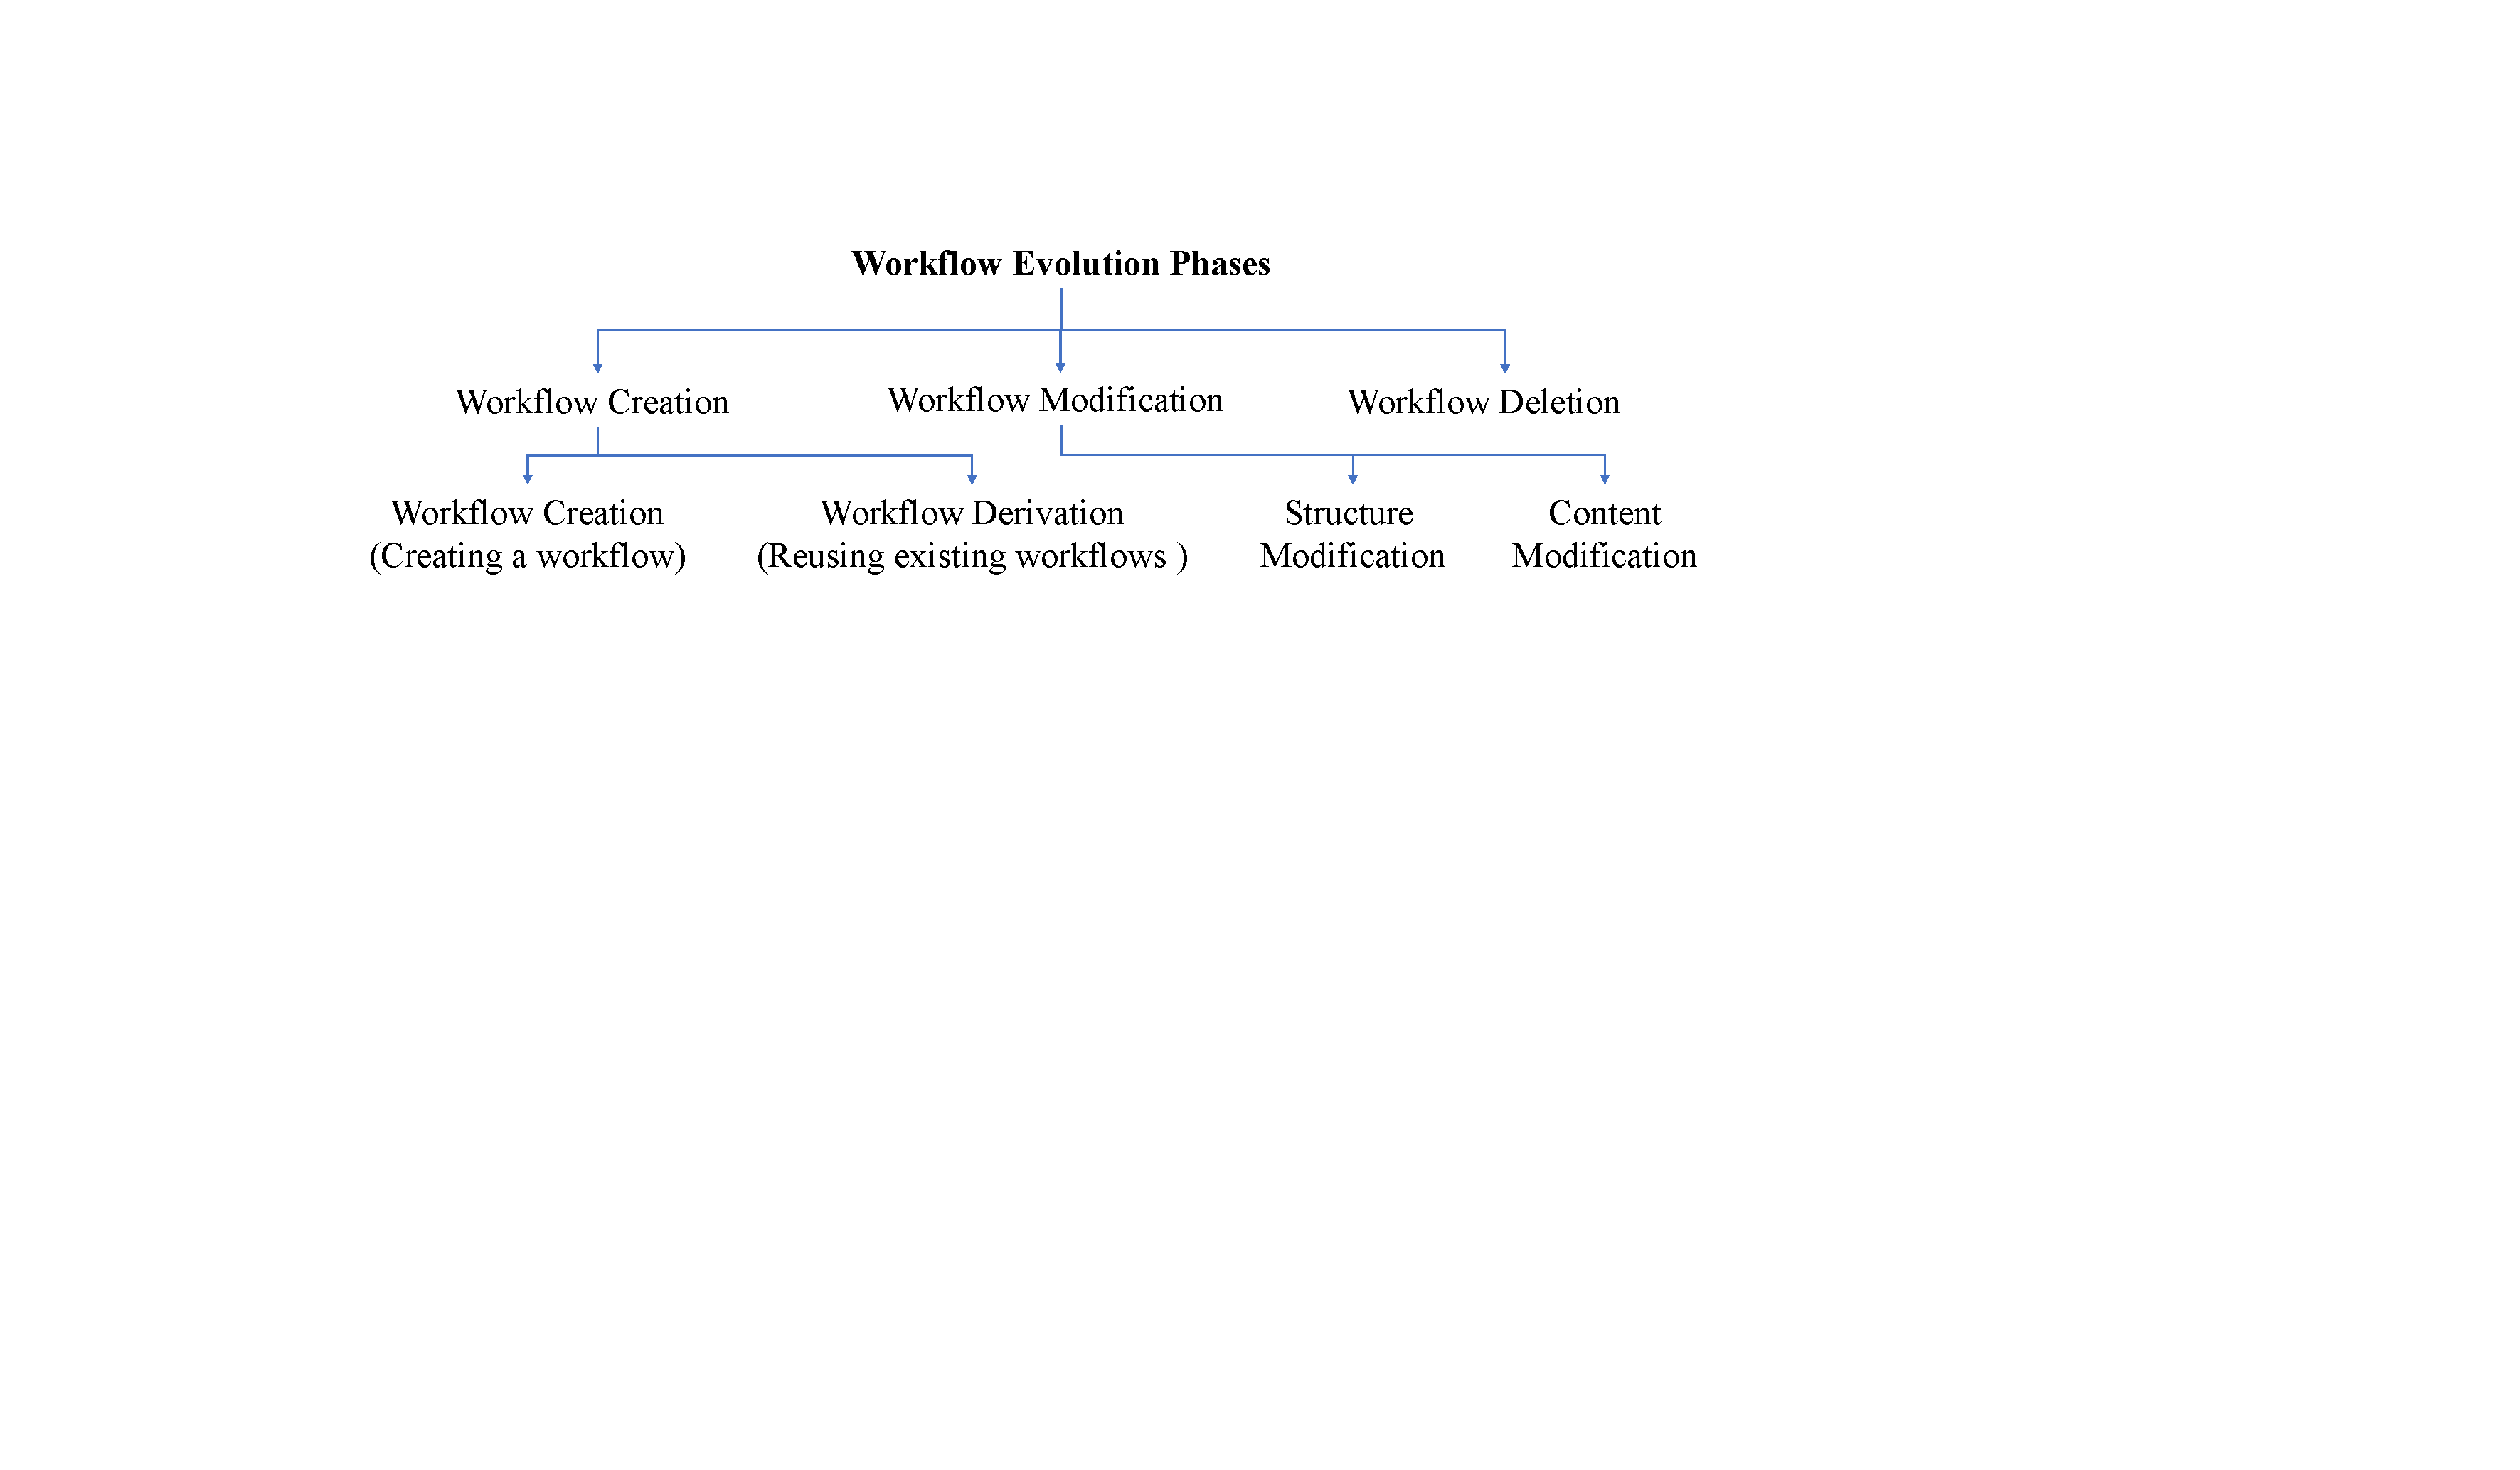
\includegraphics[width=0.8\linewidth]{figures/workflow-evolution-lifecycle.pdf}
    \caption{Workflow evolution phases}
    \label{fig:workflow-evolution}
\end{figure}

\subsubsection{Creation of the Workflow}
\label{subsec:workflow-creation}

Scientific workflows can be designed using a workflow engine. They are often not completely disjoint, and some of them may reuse other workflows. Consequently, the creation of a workflow can be done either by creating all elements of the workflow from scratch or by reusing the existing workflows.

\begin{itemize}
\item[-]\textbf{Workflow Creation:} When a workflow is designed, all its elements are created during workflow creation time. There is no derivation history for the workflow. We used generation pattern to model the workflow creation provenance. 

Figure~\ref{fig:workflow-creation-provenance} shows the provenance pattern for workflow creation. For brevity, \texttt{Workflow} here represents the workflow and its elements. \texttt{Generation} is the completion of the production of a new workflow by an activity \texttt{Creation}. This workflow does not exist before generation and becomes available for use after this generation. \texttt{Agent} is the creator of this workflow.

\begin{figure}[h]
    \centering
    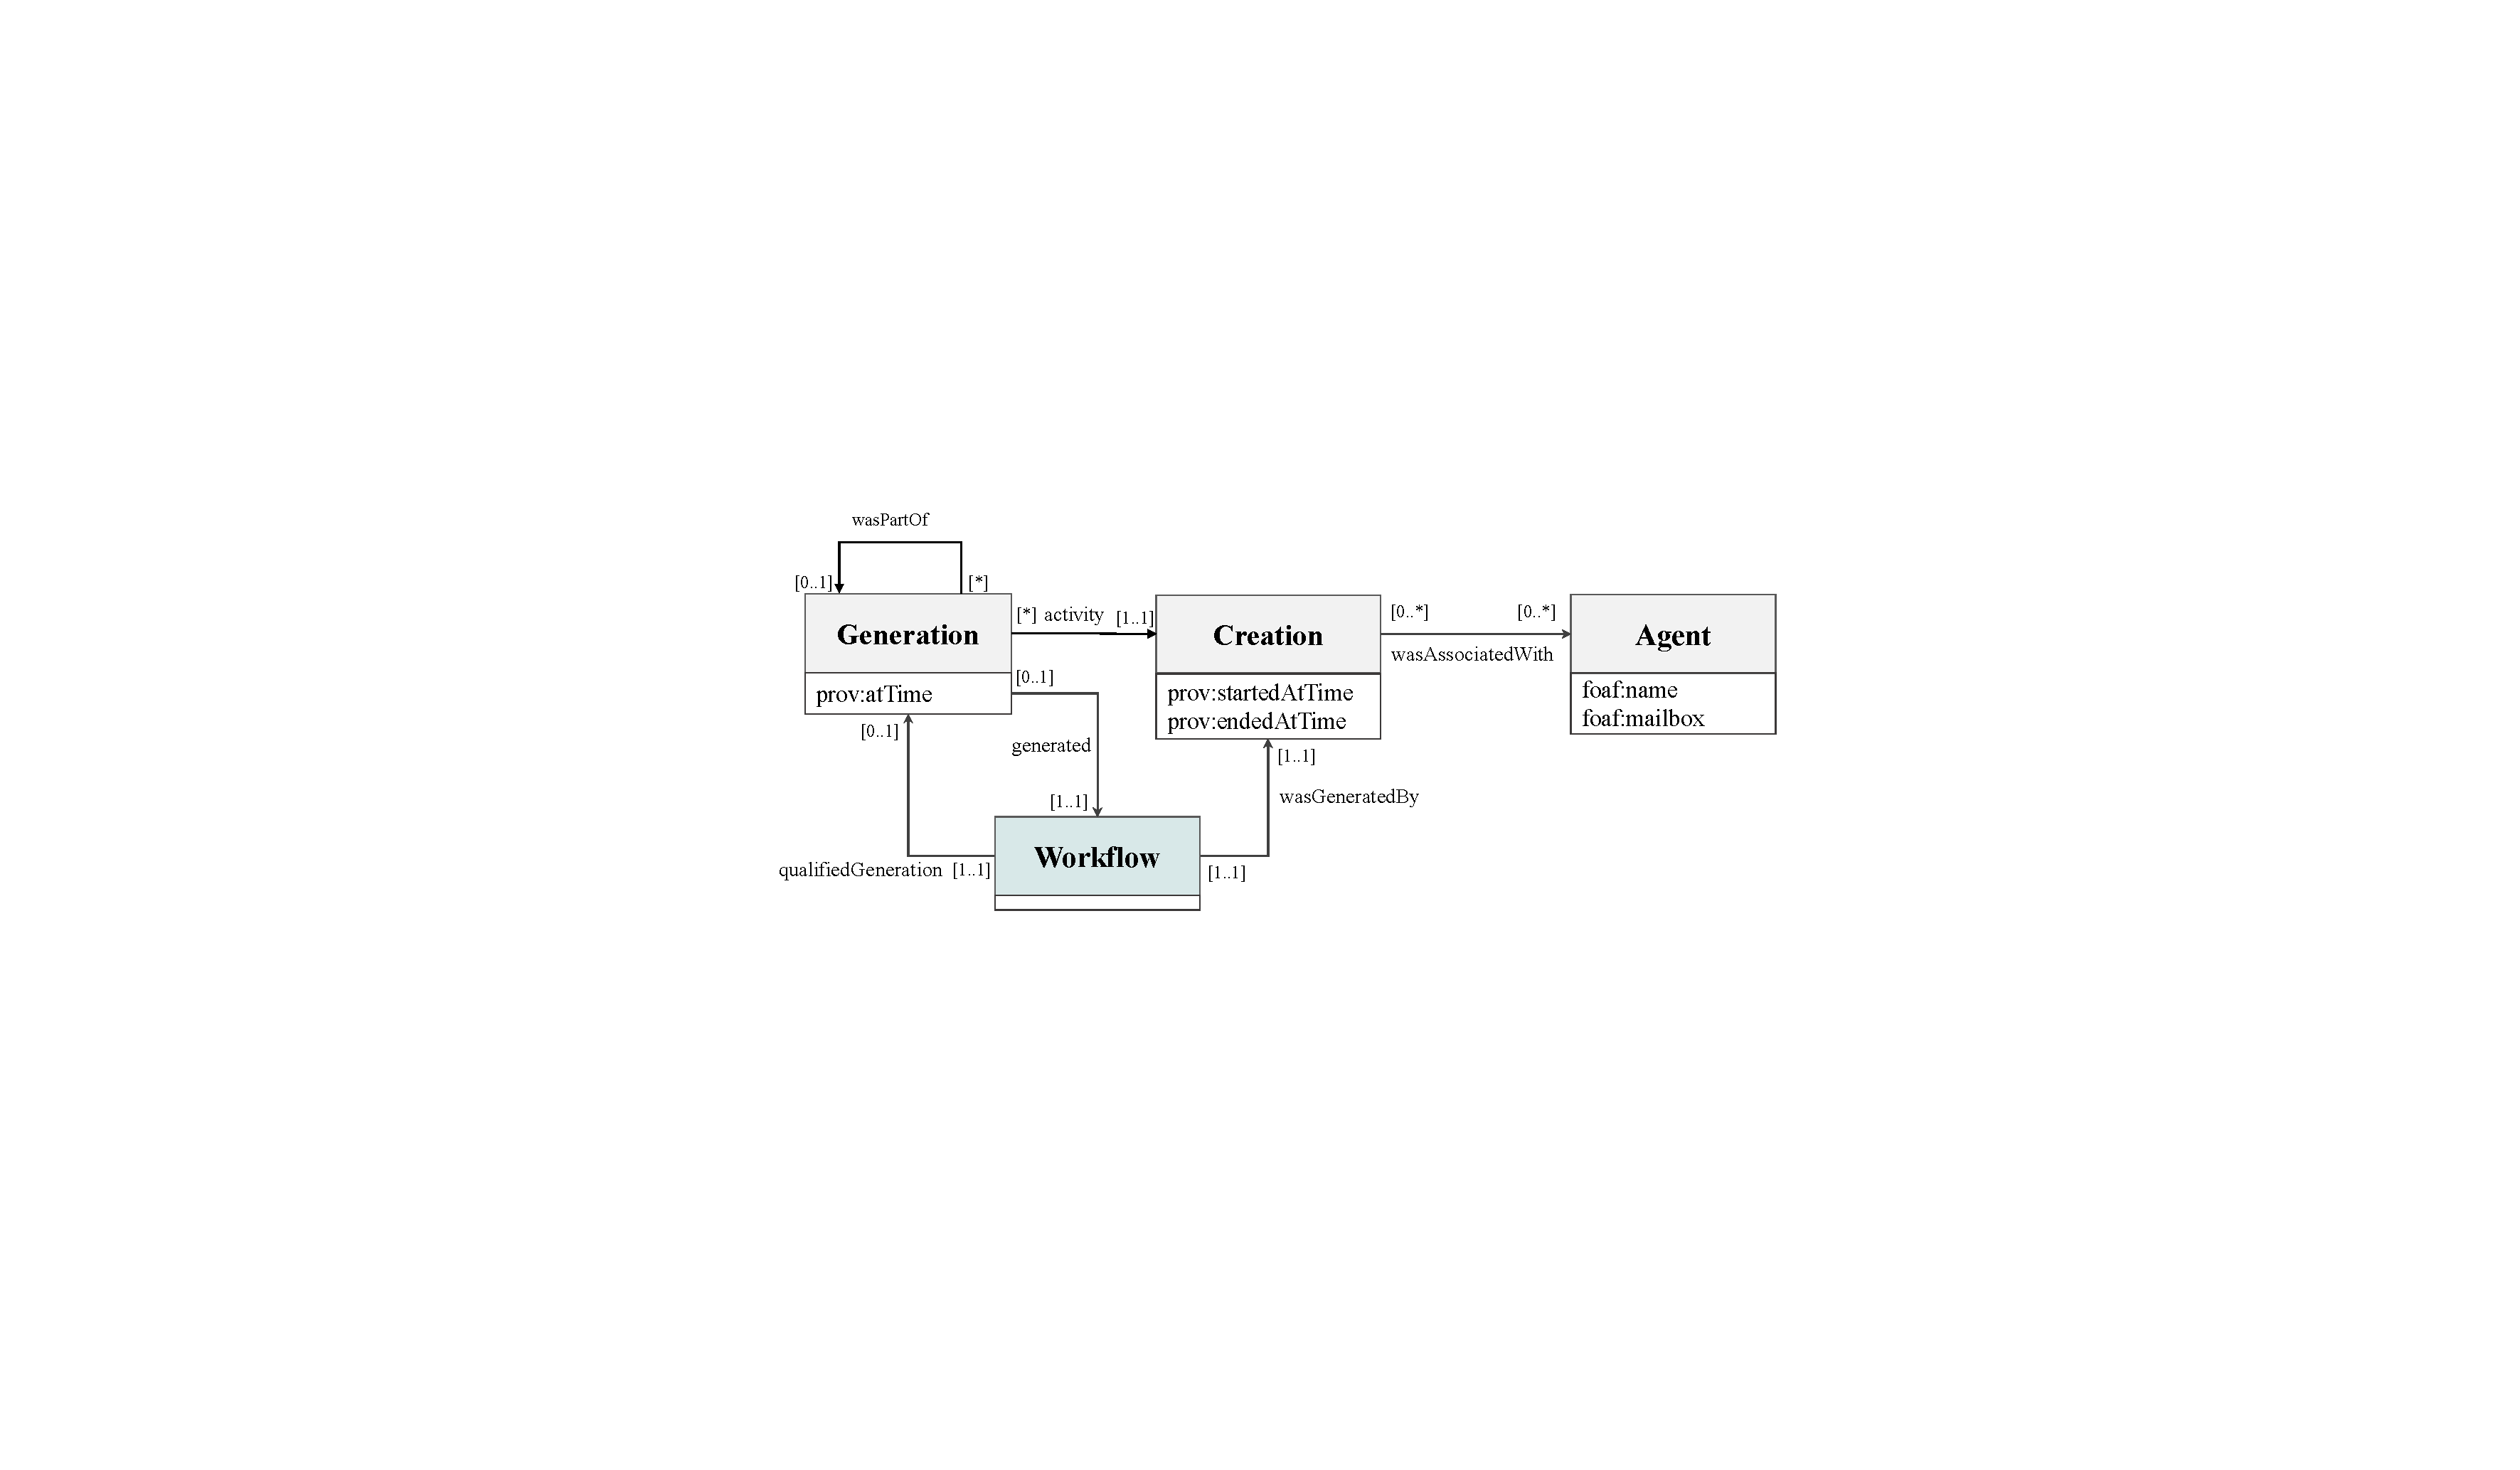
\includegraphics[width=0.7\linewidth]{figures/workflow-creation-pattern.pdf}
    \caption{Workflow Creation Provenance Pattern}
    \label{fig:workflow-creation-provenance}
\end{figure}

In creation provenance, workflow and its constituent elements will have their dedicated generation instances; therefore, multiple generations under the same creation activity may occur. However, in this case, the generation of the elements would be part of the generation of the workflow, as shown in axioms A1 and A2.  

\begin{center}
    $\forall$ $x_w$, $x_e$ : Generation,
    $\forall$ $c$ : Creation,
    activity($x_w$, $c$) $\wedge$ activity($x_e$, $c$) $\rightarrow$  wasPartOf($x_e$, $x_w$) (\textbf{A1})
\end{center}

\begin{center}
    $\forall$ $x_w$, $x_e$ : InstantaneousEvent,
    Generation($x_e$) $\wedge$ wasPartOf($x_e$, $x_w$)  $\rightarrow$ Generation($x_w$)   (\textbf{A2})
\end{center}

\item[-]\textbf{Workflow Derivation:} A workflow can be created by reusing an existing workflow referred to as workflow derivation in this paper. %When a workflow is created by reusing another workflow, the original workflow must exist and execute in its entirety; only then it can become a part of the newly created workflow.
A workflow must exist and execute in its entirety so that it can be reused while creating another workflow. 

Figure~\ref{fig:workflow-reuse-provenance} shows the provenance model for workflow creation when it is derived from another workflow. \texttt{Derivation} constructs a new workflow based on a pre-existing workflow.
%A \texttt{workflow} created from another workflow as a result of some underpinning activity/activities, referred to as \texttt{creation}, in such derivations. 
A \texttt{workflow} uses another workflow during the \texttt{creation} of the workflow in such a derivation.
In its purest form, derivation relates to two workflows where the \texttt{usage} of the \texttt{usedEntity} is provided to make the derivation path explicit.  
%To provide an entirely accurate description of the derivation, the \textit{Generation} and \textit{Usage}, of the generated and used entities, is provided, which makes the derivation path explicit through usage, activity, and generation. 

\begin{figure}[h]
    \centering
    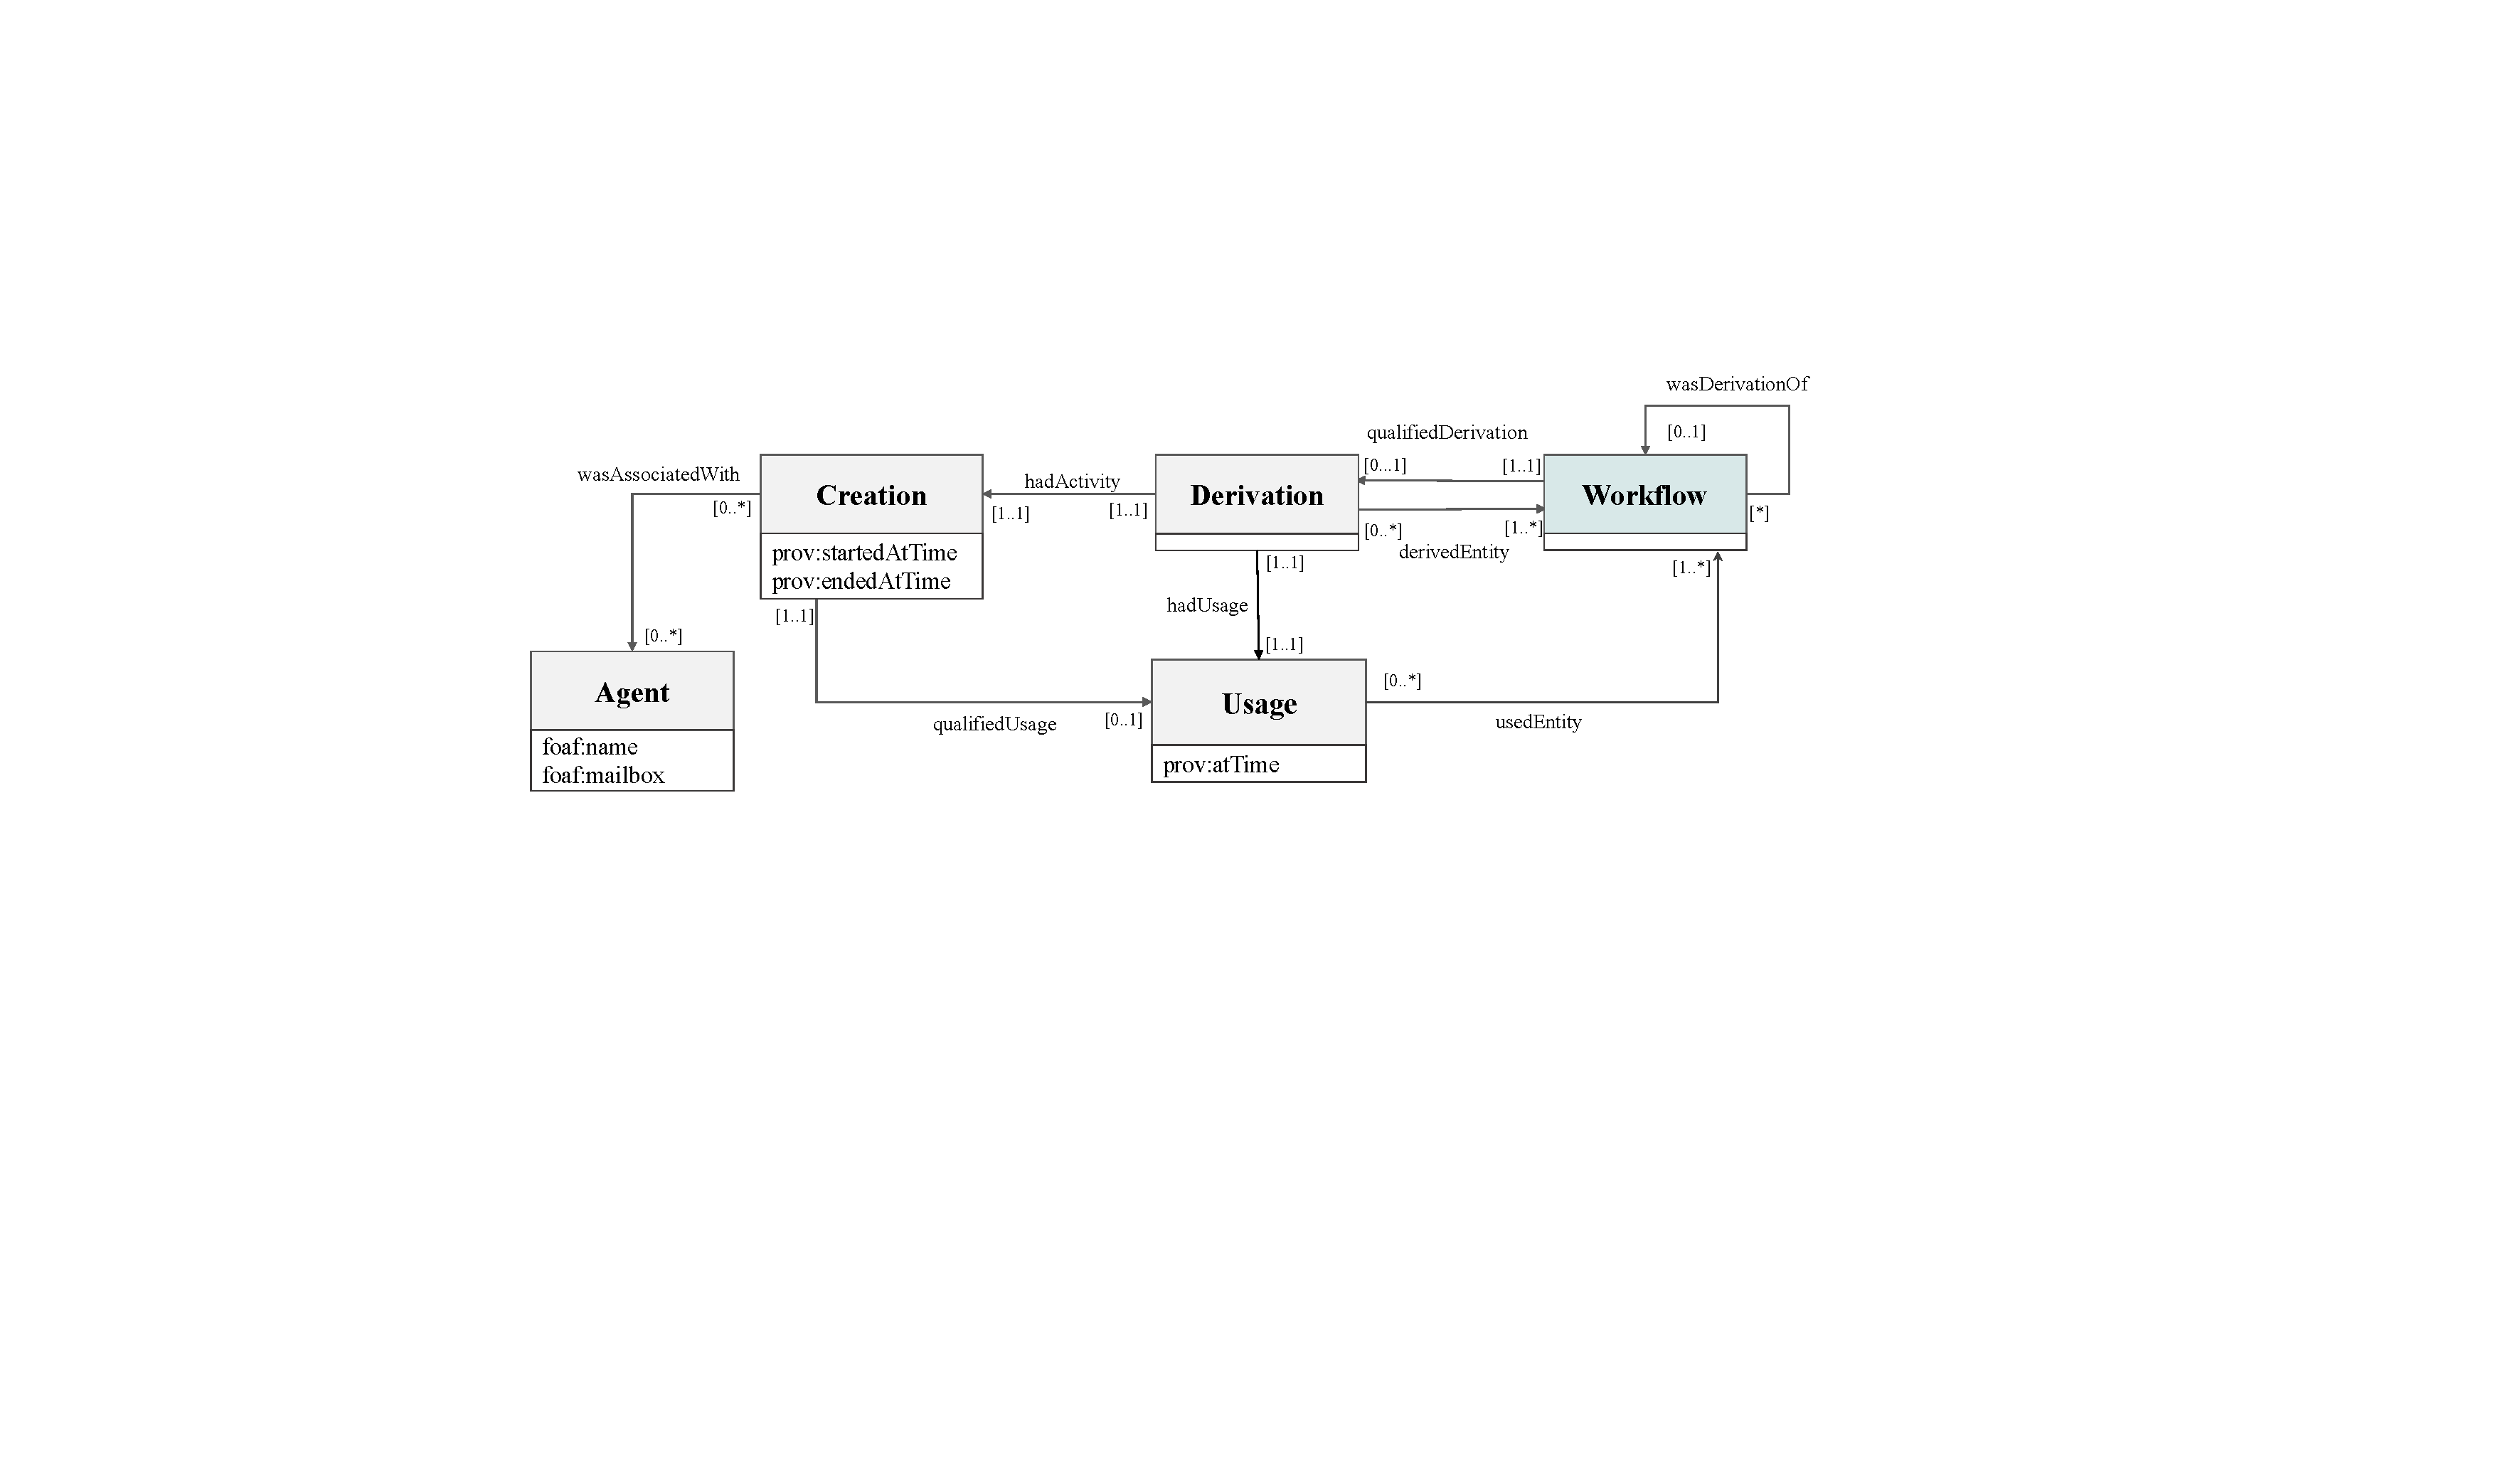
\includegraphics[width=0.85\linewidth]{figures/workflow-reuse-pattern.pdf}
    \caption{Workflow Derivation Provenance Pattern}
    \label{fig:workflow-reuse-provenance}
\end{figure}

Information such as \texttt{creation} and \texttt{usage} are linked to \texttt{derivation}, as shown in axiom A3, to aid analysis of provenance.

\begin{center}
    $\forall$ $w_i$, $w_j$ : Workflow,
    $\forall$ $d$ : Derivation,
    $\forall$ $u$ : Usage,
    qualifiedDerivation($w_i$,$d$) $\wedge$ hadUsage($d$,$u$) $\wedge$ usedEntity($u$,$w_k$) $\rightarrow$ wasDerivationOf($w_i$,$w_j$) \textbf{(A3)}
\end{center}

Moreover, the derivation is transitive, i.e.,   
\begin{center}
    $\forall$ $w_i$, $w_j$, $w_k$ : Workflow,
    wasDerivationOf($w_i$,$w_j$) $\wedge$ wasDerivationOf($w_j$,$w_k$) $\rightarrow$ wasDerivationOf($w_i$,$w_k$) \textbf{(A4)}
\end{center}

Finally, for all workflows there should be either a derivation or a generation provenance record i.e., 

\begin{center}
    $\forall$ $w$ : Workflow,
    $\exists$ $c$ $\mid$ $c$ : Creation $\wedge$
     ( wasGeneratedBy($w$,$c$) $\oplus$ ( qualifiedDerivation(w,d) $\wedge$ hadActivity(d,c)) \textbf{(A5)}
\end{center}
\end{itemize}

\subsubsection{Deletion of the Workflow}
\label{subsec:workflow-deletion}

The suppression or deletion of a workflow is handled by invalidation of that workflow. 
This makes the workflow unavailable for further use, but it is accessible to explore the evolution of a workflow. We used invalidation concept from PROV-DM to model a workflow deletion provenance pattern. 
Figure~\ref{fig:workflow-deletion} shows the provenance pattern for workflow deletion. For brevity, \textit{Workflow} here represents the workflow and(or) its elements. \texttt{Invalidation} is the start of the cessation or expiry of an existing workflow by a \texttt{Deletion} activity. The workflow is no longer available for the use after invalidation. Any generation or usage of a workflow precedes its invalidation. A \texttt{Deletion} is associated with an \texttt{Agent}.

\begin{figure}[h]
    \centering
    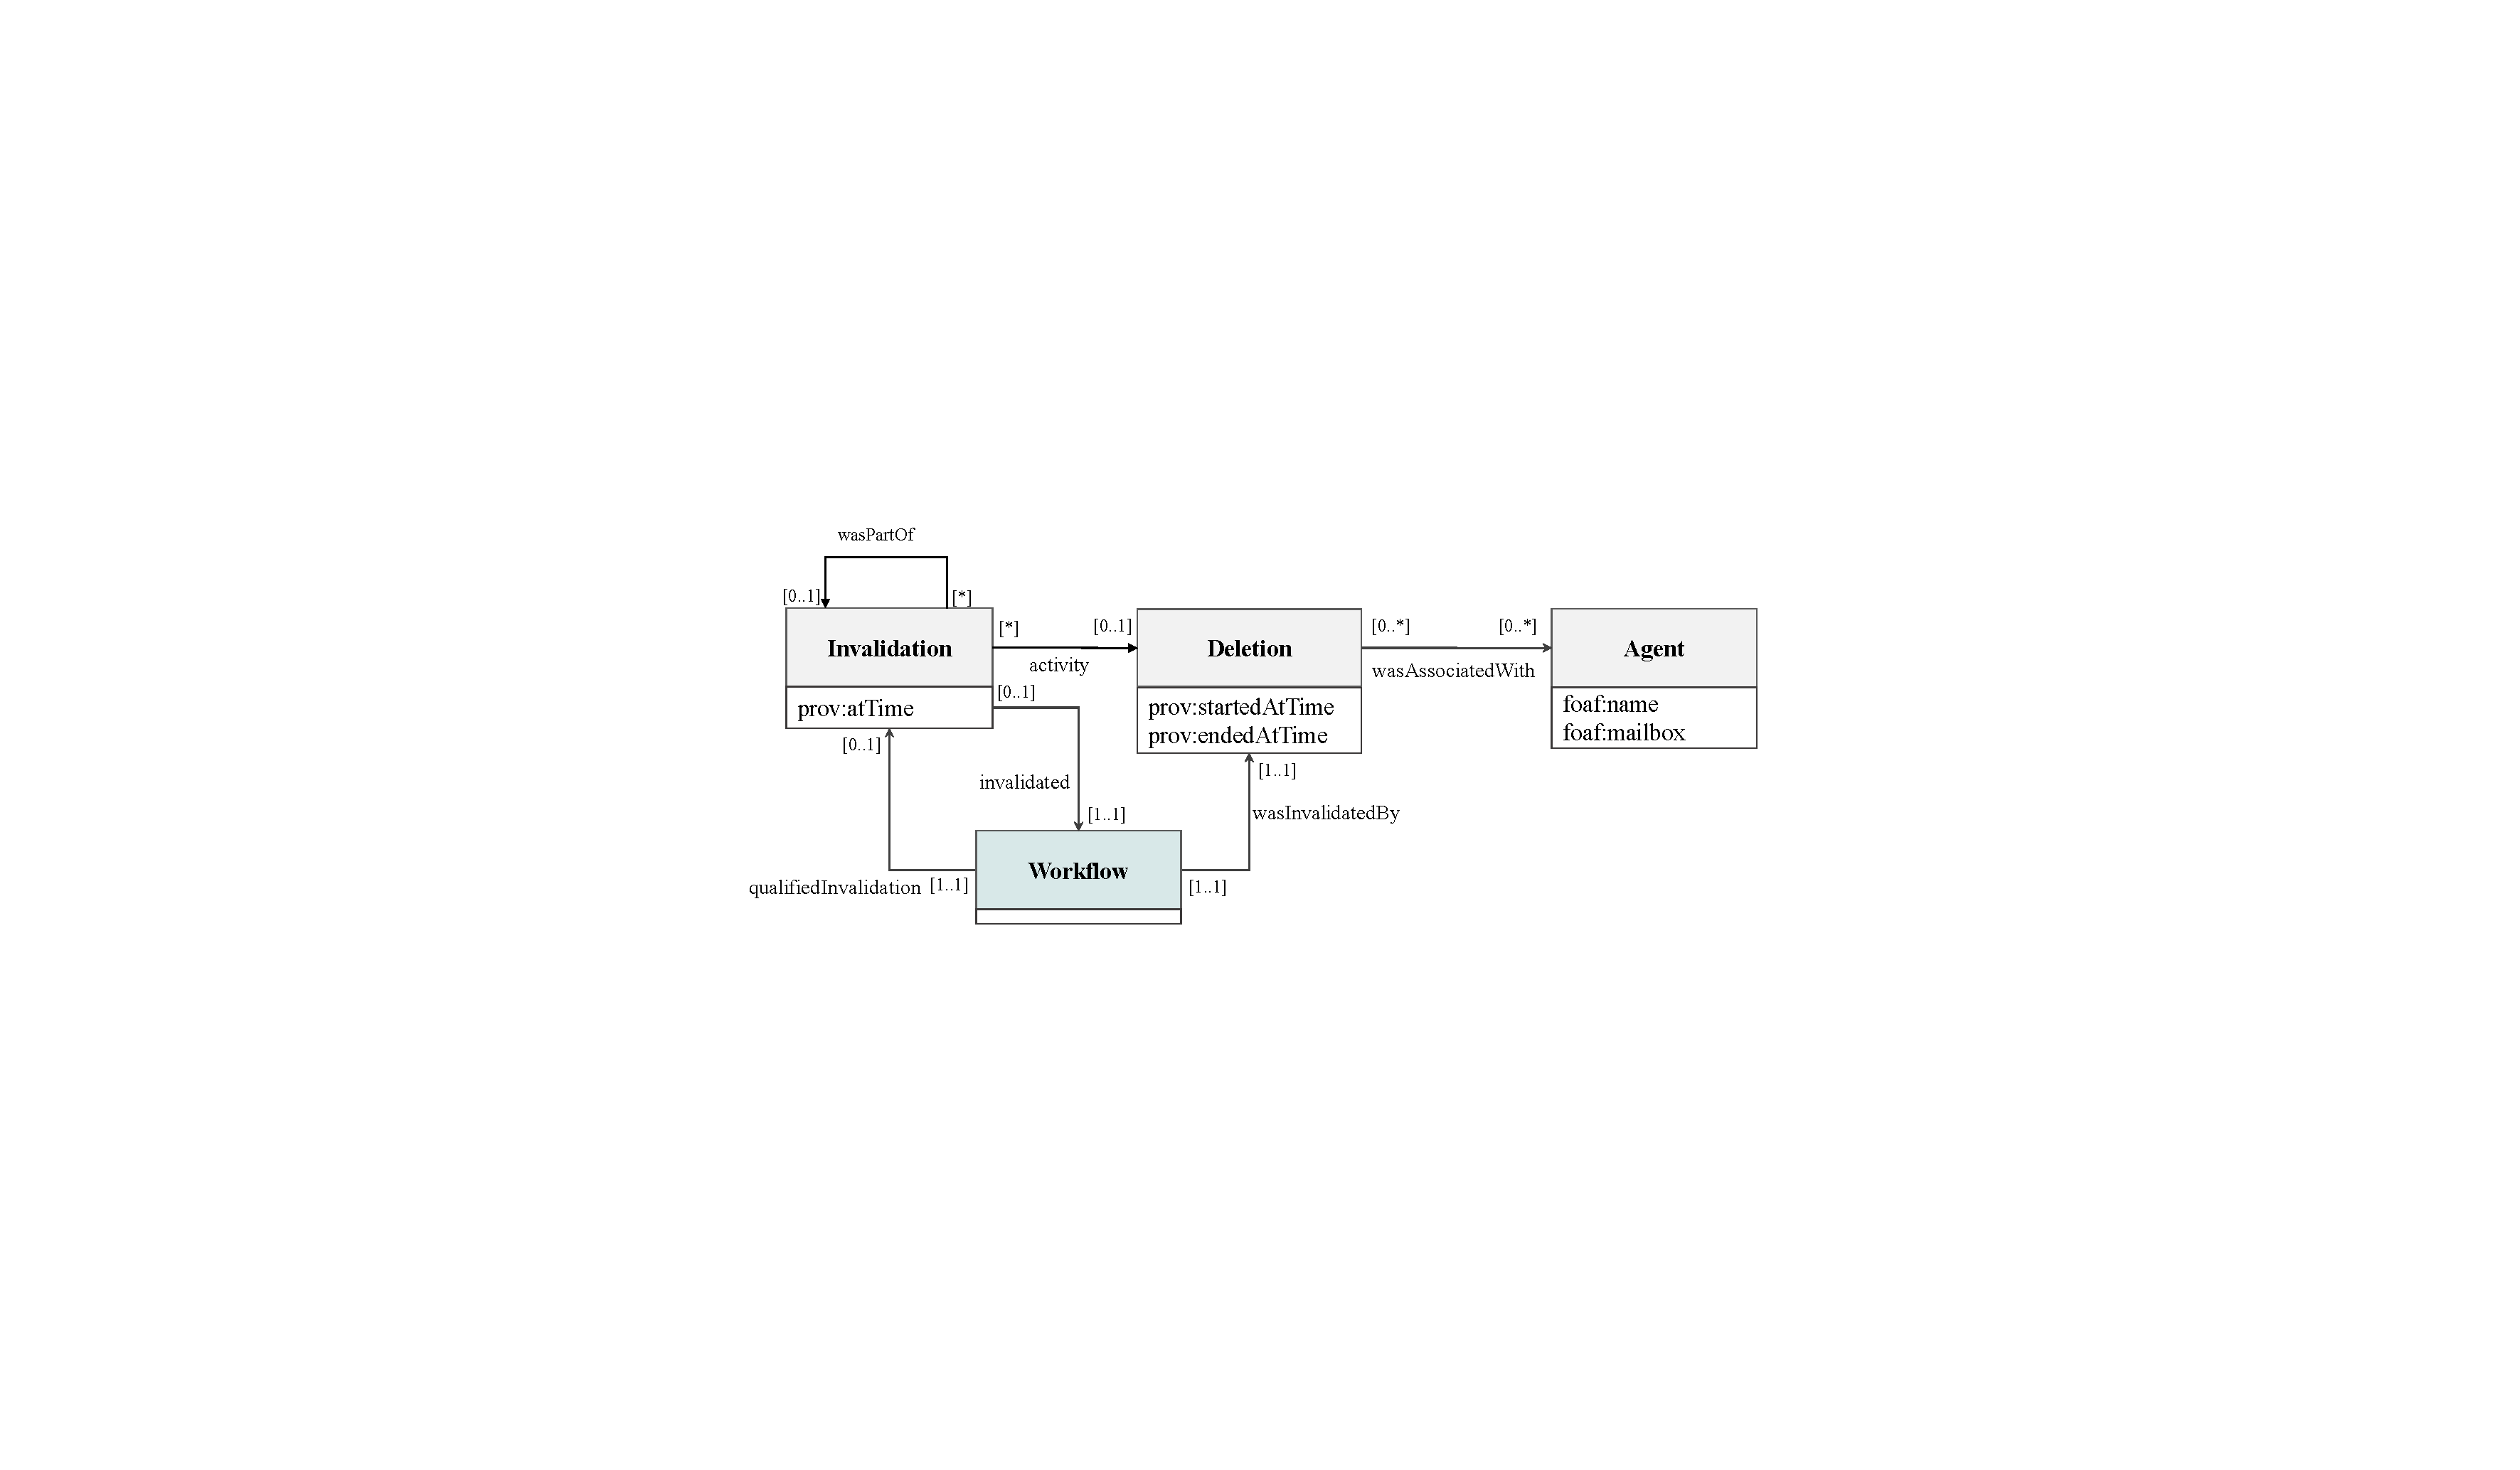
\includegraphics[width=0.7\linewidth]{figures/workflow-deletion-pattern.pdf}
    \caption{Workflow Invalidation Provenance Pattern}
    \label{fig:workflow-deletion}
\end{figure}

When a workflow is invalidated, all its elements are invalidated as a part of the workflow deletion activity, as described in A5.

\begin{center}
    $\forall$ $x_i$, $x_j$ : $Invalidation$,
    $\forall$ $w$ : Workflow,
    $\forall$ $p$ : Program $\cup$ Controller $\cup$ Port $\cup$ Channel $\cup$ Parameter, 
    $p$ $\in$ $w$ $\wedge$ qualifiedInvalidation($w$, $x_i$) $\rightarrow$  qualifiedInvalidation($p$, $x_j$) $\wedge$ wasPartOf($x_j$, $x_i$) (\textbf{A5})
\end{center}


The workflow and its elements have their dedicated invalidation instances and the invalidation event of elements is a part of workflow invalidation, as shown in axioms A6 and A7.  

\begin{center}
    $\forall$ $x_i$, $x_j$ : InstantaneousEvent,
    Invalidation($x_i$) $\wedge$ wasPartOf($x_j$, $x_i$)  $\rightarrow$ Invalidation($x_i$)   (\textbf{A6})
\end{center}

\begin{center}
    $\forall$ $x_i$, $x_j$ : Invalidation,
    $\forall$ $d$ : Deletion,
    activity($x_i$, $d$) $\wedge$ activity($x_j$, $d$) $\rightarrow$  wasPartOf($x_i$, $x_j$) $\vee$ wasPartOf($x_j$, $x_i$) (\textbf{A7})
\end{center}



\subsubsection{Modification of the Workflow}
\label{subsec:workflow-modification}

Workflows are likely to be modified due to different reasons, and there is a need to manage the modification provenance. 
\begin{figure}[h]
    \centering
    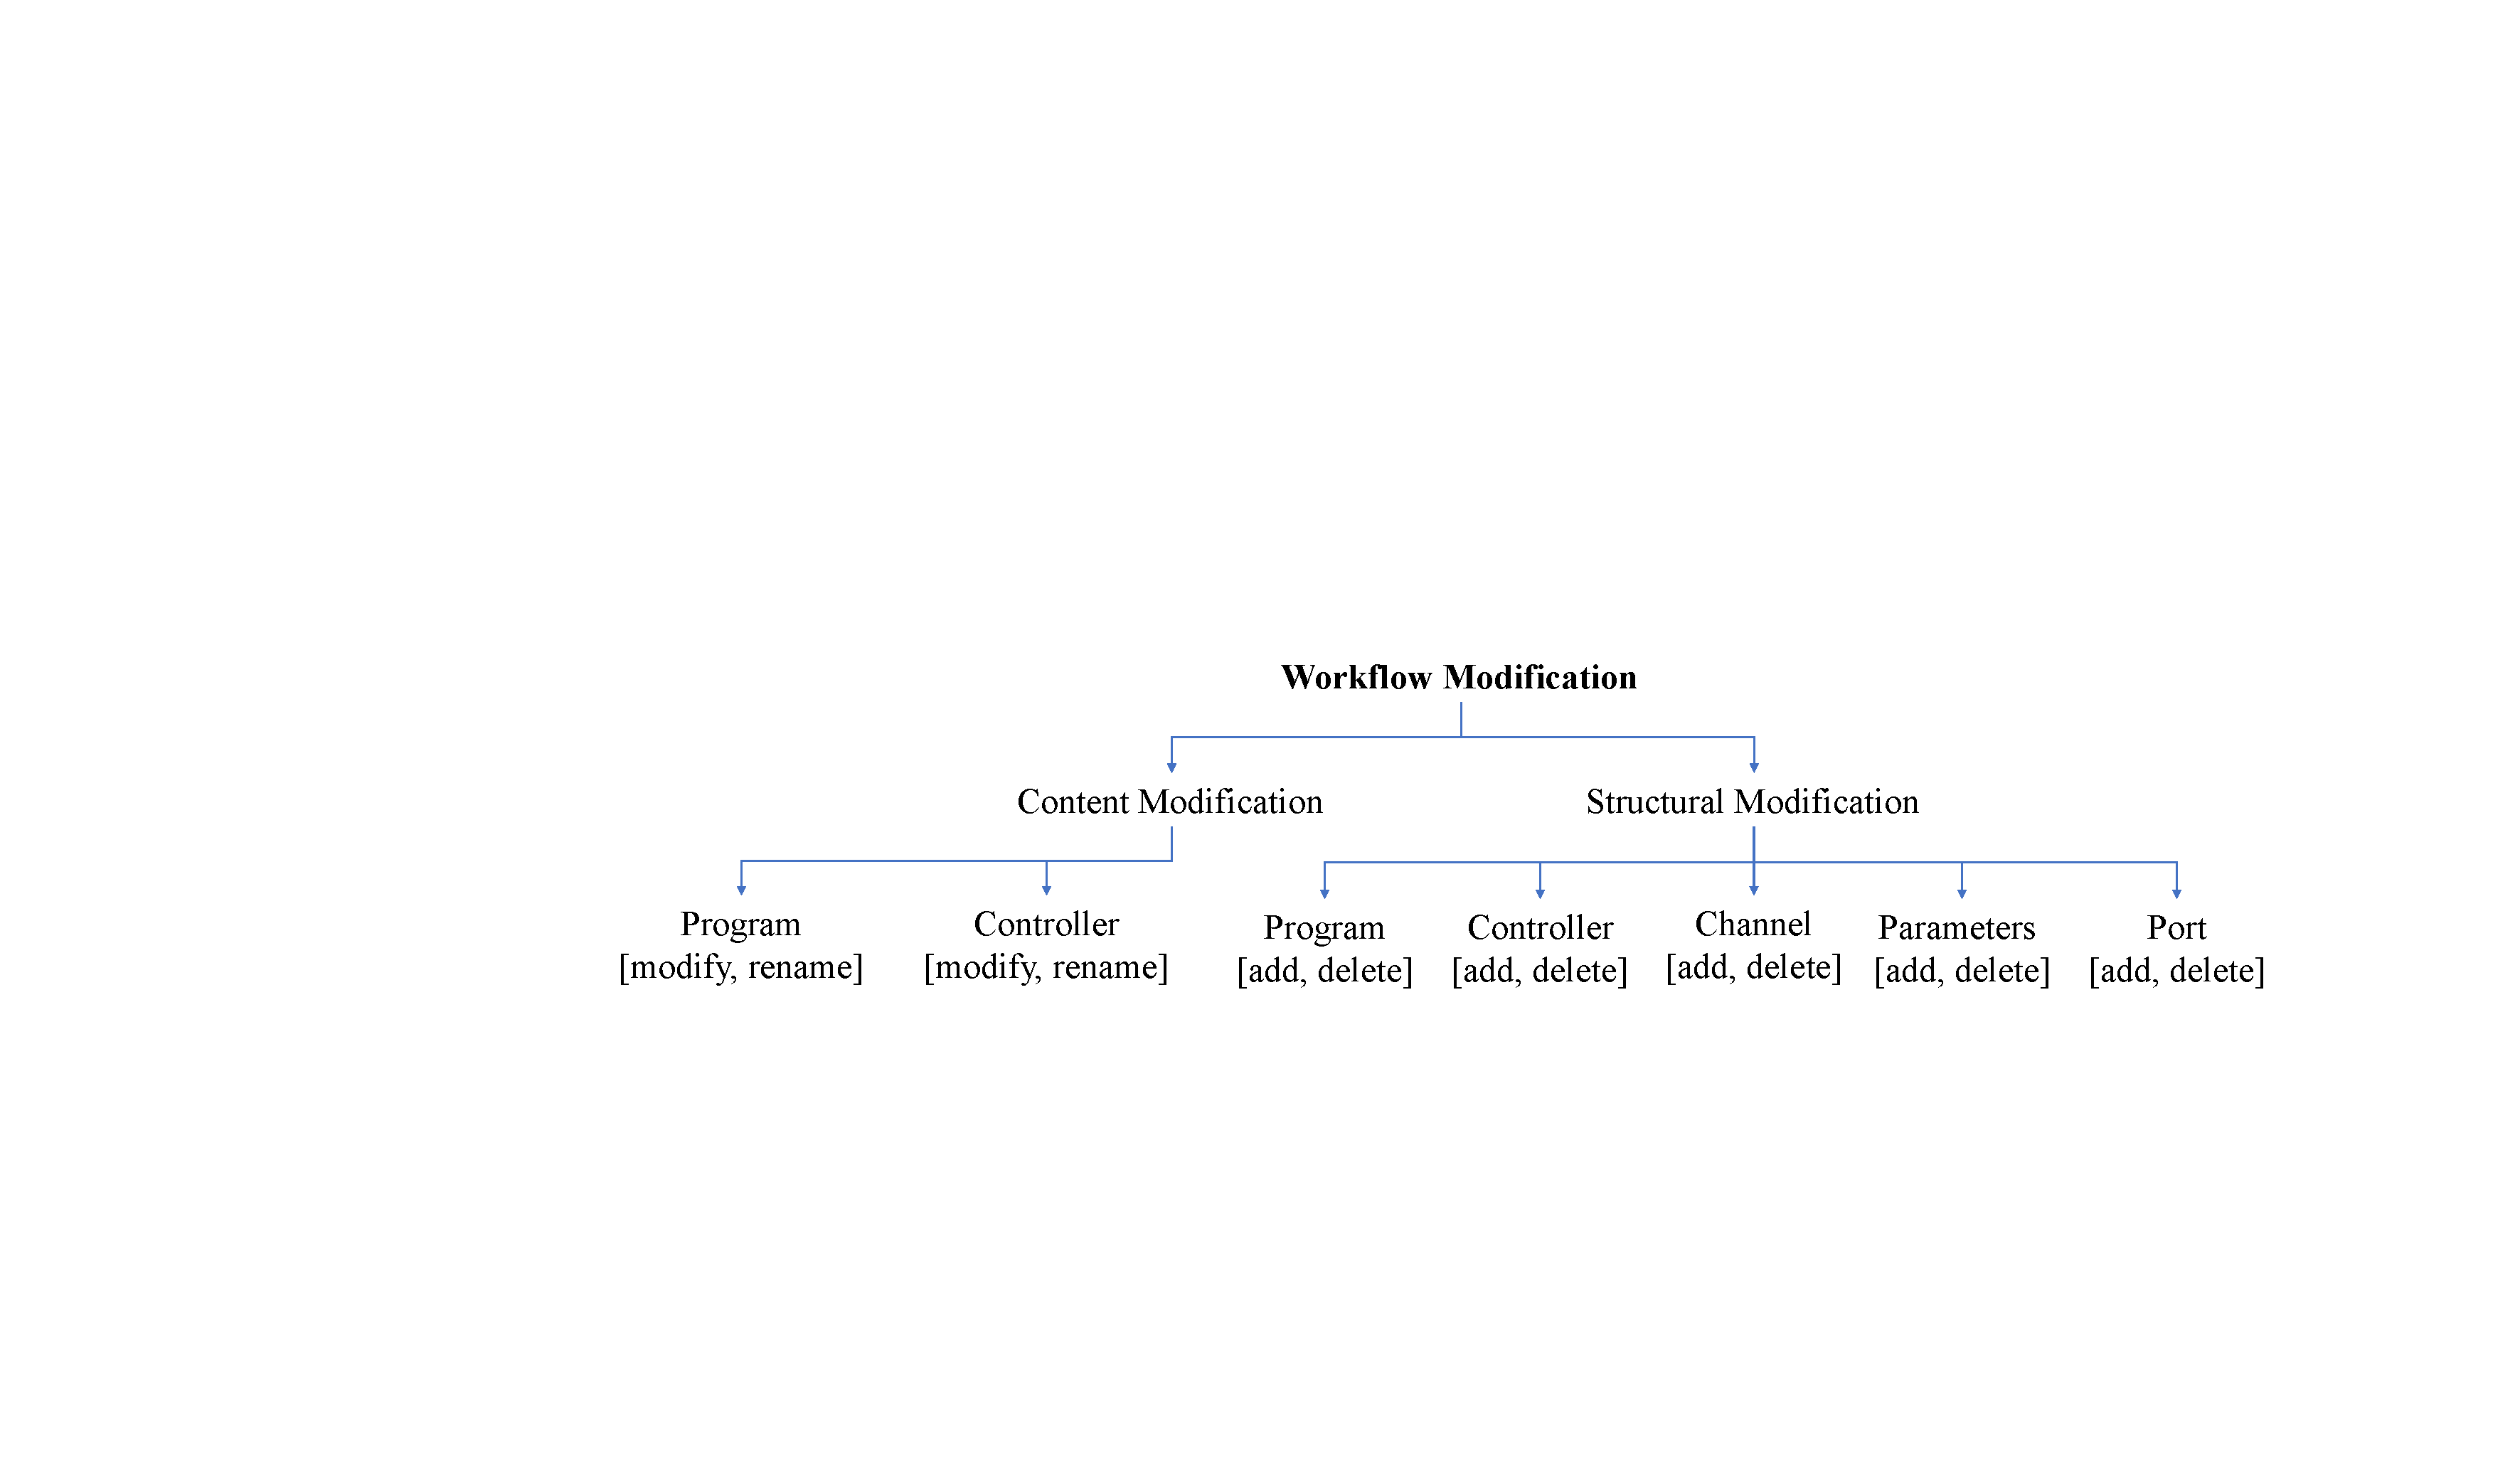
\includegraphics[width=0.8\linewidth]{figures/workflow-modification.pdf}
    \caption{Possible Modification types in Workflows}
    \label{fig:workflow-modification}
\end{figure}

Two types of modifications might affect a workflow i.e., a change in workflow structure or its contents. Modifications in workflow structure includes the addition or suppression of a Program, Controller, Channel, Parameter, or Port. 
%Modifications in workflow structure includes the addition of a program, addition of a controller, suppression of a program, suppression of a controller. 
Whereas, modification in workflow contents includes modification of a Program. 
Moreover, a workflow can be modified as a result of a single change in the workflow or composite changes, which may include structural and content changes in a modification activity. A hierarchy of possible modifications in a workflow is designed considering the given aspects, as shown in Figure~\ref{fig:workflow-modification}.  This figure shows the elements of a workflow and type of operations (i.e., add, delete, modify and rename) that are relevant with reference to workflow modification.

Here, addition and deletion of a workflow or its elements (i.e., Program, Controller, Channel, or Parameter) represent a structural modification. Whereas, modifying and renaming these components are content modifications. Moreover, modifying a Program includes modifying or renaming a model (i.e., Program content modification) or adding, deleting, and renaming Ports (i.e., Program interface modification).

A workflow modification provenance pattern is presented in Figure~\ref{fig:workflow-modification-provenance} based on the possible modifications in workflows. 

\begin{figure}[h]
    \centering
    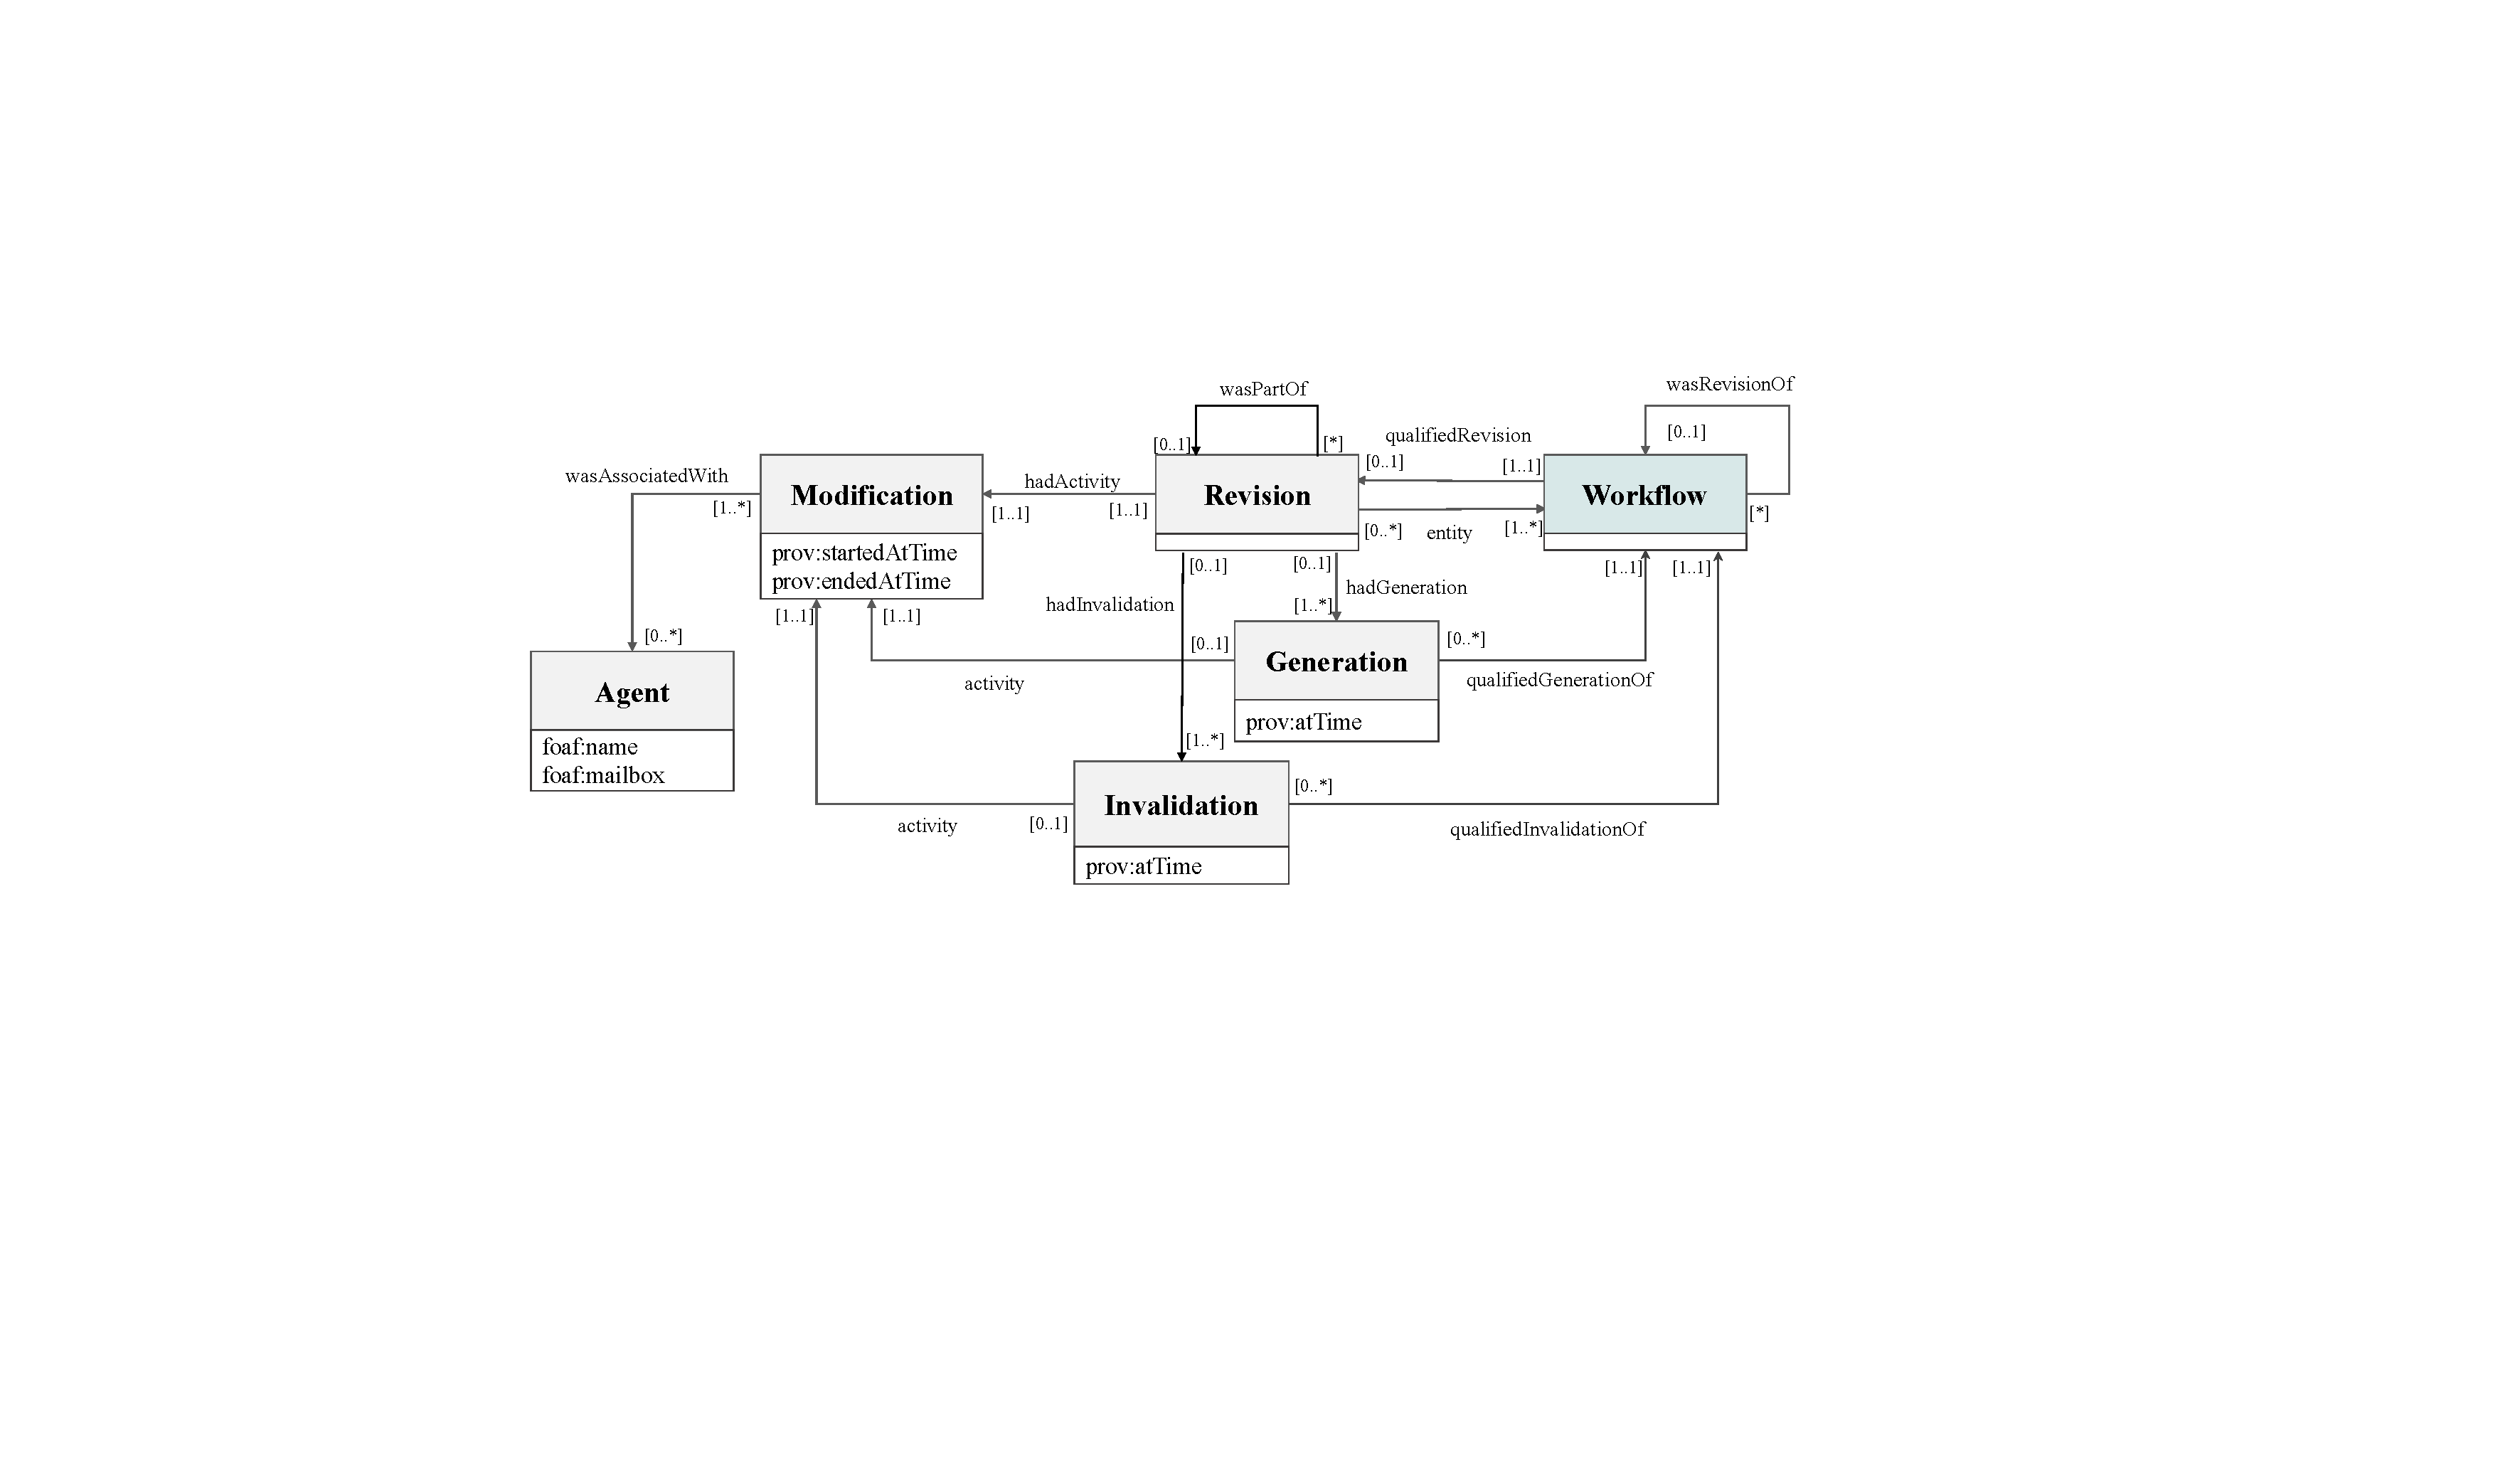
\includegraphics[width=0.95\linewidth]{figures/workflow-modification-pattern.pdf}
    \caption{Workflow Modification Provenance Pattern}
    \label{fig:workflow-modification-provenance}
\end{figure}

A \texttt{Revision} is a derivation of a workflow for which the resultant workflow is a revised version of some original workflow and contains substantial content from the original. %A \texttt{Workflow} created from another workflow as a result of some activity/activities \texttt{Modification} in such revisions. 
Revision relates two workflows where a revised workflow is the latest version of the workflow. The implication here is that revision results in the generation of a new version of the workflow while invalidating the original one. This new version of the workflow is the \textit{current} version. While the \textit{previous} version is not deleted, rather it becomes invalidated. To provide a completely accurate description of the revision, the \texttt{Generation} and \texttt{Invalidation} of the generated and invalidated entities are provided. We then make the derivation path explicit through activity, generation, and invalidation. Linking such information with revision aids analysis of provenance and facilitates moving backward and forward in revised workflows history.

Revision is transitive just like derivation, i.e.,   
\begin{center}
    $\forall$ $w_i$, $w_j$, $w_k$ : Workflow,
    wasRevisionOf($w_i$,$w_j$) $\wedge$ wasRevisionOf($w_j$,$w_k$) $\rightarrow$ wasRevisionOf($w_i$,$w_k$) \textbf{(A8)}
\end{center}


A workflow revision represents the composite changes in a workflow. However, a composite change (workflow modification) is an aggregation of atomic changes, i.e., modification in the elements (programs, controllers, channels, and parameters), as shown in Figure~\ref{fig:workflow-modification}. 
While a composite change is captured through revision pattern shown in Figure~\ref{fig:workflow-modification-provenance}, atomic changes can be captured differently based on the modification operator. For example,

\begin{itemize}
\item[-] \textit{Addition:} adding a component in a workflow during a revision is captured by \textbf{creation pattern} shown in Figure~\ref{fig:workflow-creation-provenance}.
\item[-] \textit{Deletion:} Our interest is in managing the evolution of a workflow; therefore, instead of deleting a workflow or its component the suppression or deletion is represented with \textbf{invalidation pattern} as shown in Figure~\ref{fig:workflow-deletion}. 
\item[-] \textit{Modification:} modifying a component is a revision of original component in a workflow, therefore, is captured by the \textbf{modification pattern} shown in Figure~\ref{fig:workflow-modification-provenance}. A component revision is envisioned as a part of a workflow revision.
\item[-] \textit{Renaming:} renaming is captured through the same \textbf{modification pattern}, however, the activity that handles renaming will distinguish it from modification. 
\end{itemize}

\subsection{Workflow Evolution Provenance Ontology}
\label{subsec:evolution}

\begin{figure}[htpb]
\centering
    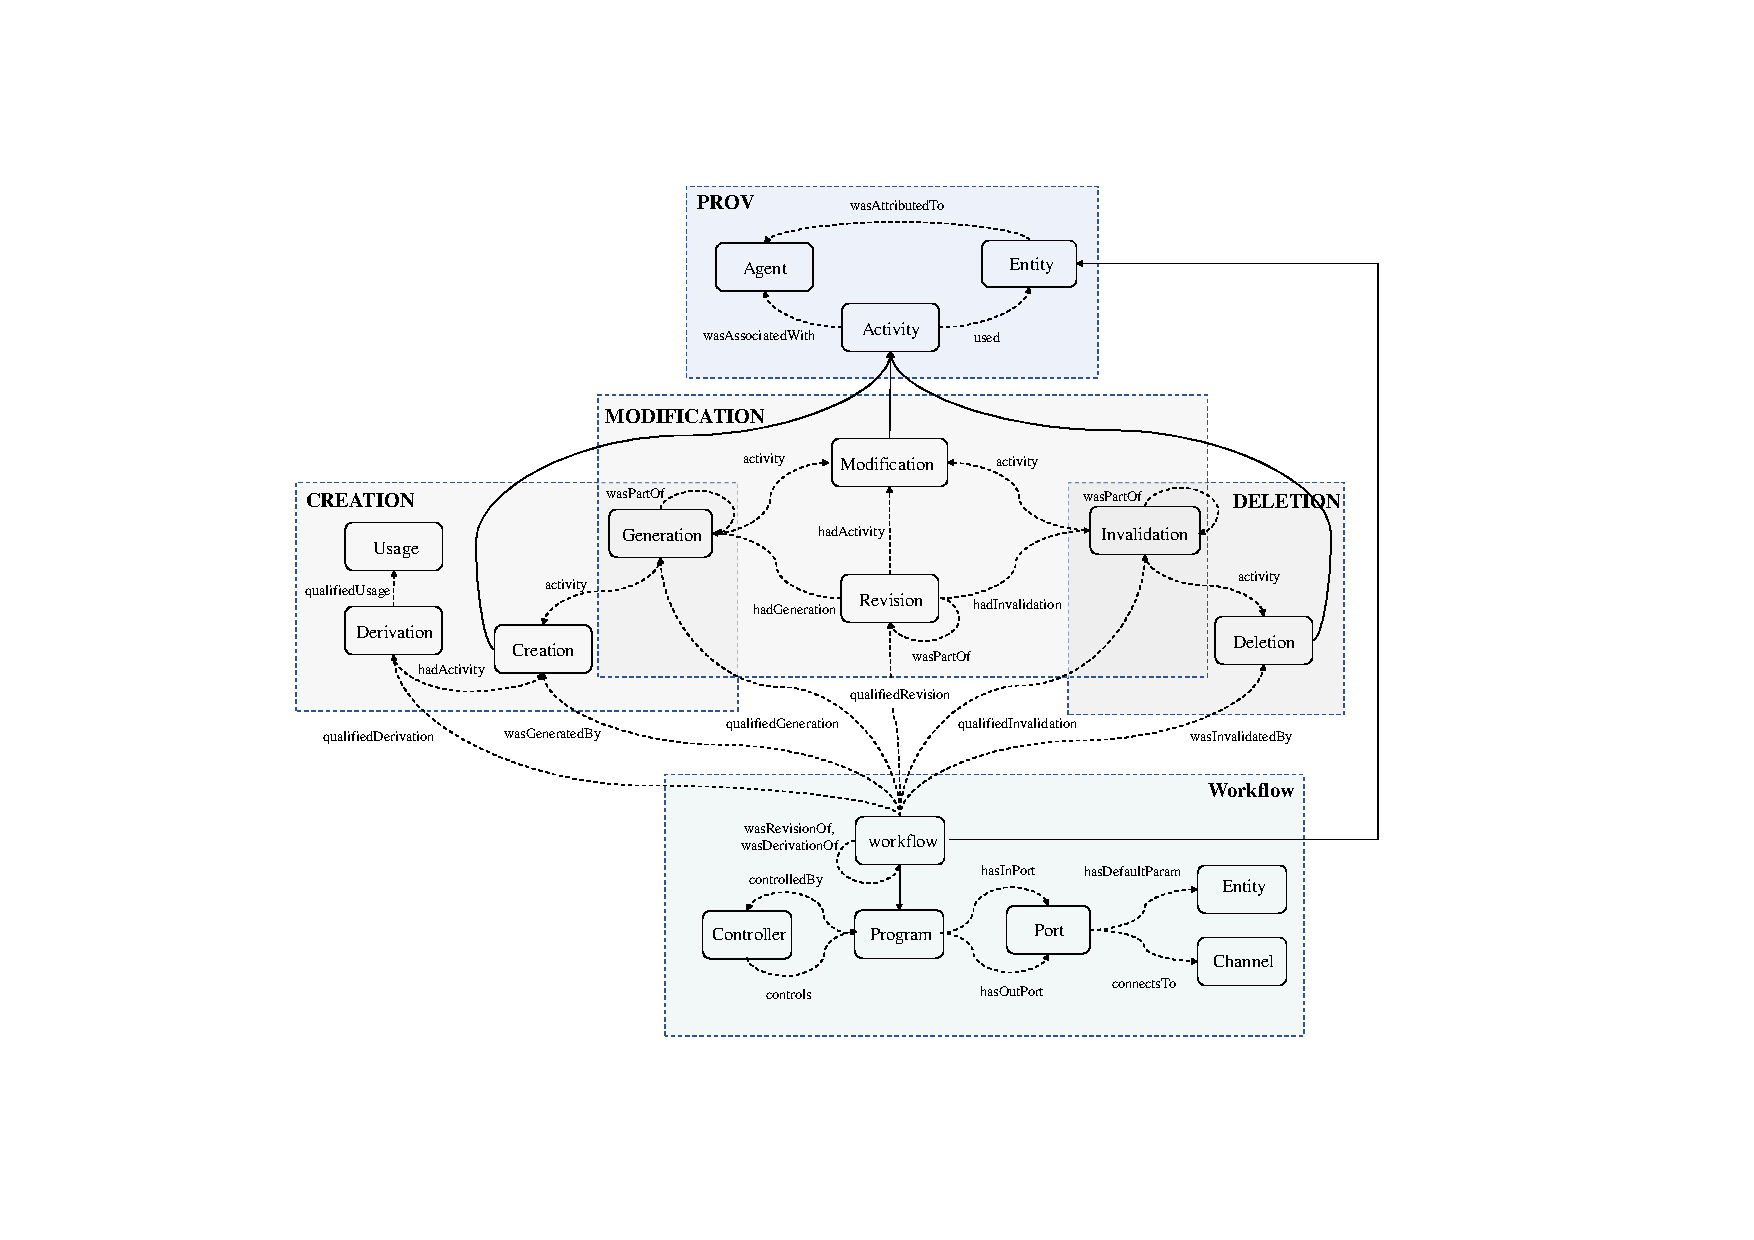
\includegraphics[width=1.0\linewidth]{figures/workflow-evolution-model.pdf}
    \caption{The workflow evolution model and its relationship to PROV}
    \label{fig:worklfow-evolution-model}
\end{figure}

In previous sections, we considered PROV as a baseline and built an extension that accommodates the need for workflow evolution-based provenance. The corresponding OWL representation of the WePROV ontology is available here\footnote{\url{https://github.com/anilabutt/WePROV-Workflow-Evolution-Provenance-Ontology/blob/master/Ontology/weprov.owl}}. Now, we present the key classes and relationships, which form the \textbf{W}orkflow \textbf{E}volution \textbf{Prov}enance Ontology. 
The proposed ontology has a workflow-centric perspective and revolves around the creation, deletion, modification, and renaming of workflows and its different elements. However, the modelling of workflows evolution aligns with the PROV-O ontology.

Figure~\ref{fig:worklfow-evolution-model} shows the ontology structure underlying all the four modelling perspectives. The colour of the classes and properties represent their participation in one or more patterns presented in Sections~\ref{subsec:workflow-creation},~\ref{subsec:workflow-deletion}, and~\ref{subsec:workflow-modification}. In this figure, \textbf{workflow} represents a complete workflow or its elements. % (i.e., \textit{program}, \textit{controller}, \textit{port}, \textit{channel} and \textit{parameter}).  
The activities of \textbf{creation}, \textbf{deletion}, \textbf{modification} and \textbf{renaming} participates in the evolution by \textbf{generation}, \textbf{usage}, and \textbf{invalidation} of workflows and its components, each performed by an \textbf{agent} and is started and ended at a time. \textbf{Derivation} uses some workflows to generate some new workflows, whereas \textbf{revision} invalidates elements of workflows to generate their new versions. 

\section{Evaluation}
\label{sec:evaluation}

The evaluation of the ontology comprises activities of \textit{validation} and \textit{verification} by ensuring that the ontology can represent real-world situation and satisfies their requirements.

\subsection{WePROV Verification}
\label{verification}
For ontology verification, SABiO~\citep{de2014sabio} suggests identifying whether the elements that make up the ontology can answer the raised competency questions. For verification, we implemented WePROV in formal ontological language OWL which allows creating SPARQL queries for testing our ontology by instantiating the competency questions on realistic examples. Listing~\ref{CQ5} presents the SPARQL query for CQ4. 
The SPARQL queries for the raised competency questions (cf. Sect. \ref{subsubsection:CQ}), showing which concepts and relations are used to answer a CQ is available here\footnote{\url{https://github.com/anilabutt/WePROV-Workflow-Evolution-Provenance-Ontology/blob/master/CompetencyQuestions/SPARQL-for-CQs.txt}}. 

\begin{lstlisting}[frame=single, linewidth=0.99\columnwidth, xleftmargin=3cm, xrightmargin=3cm, language=sparql, basicstyle=\scriptsize, caption={Which is the most unstable component of the workflow?} , label={CQ5}]
PREFIX provone:<http://purl.dataone.org/provone/2015/01/15/ontology#> 
PREFIX prov:<http://www.w3.org/ns/prov#> 
PREFIX weprov:<http://www.csiro.au/digiscape/weprov#> 

CONSTRUCT {?workflowId weprov:hasRevisions ?revisions}  
FROM <http://weprov.csiro.au/evolution/> 
WHERE {
	SELECT ?workflowId ( MAX(?revCount) AS ?revisions)  
	FROM <http://weprov.csiro.au/>
	FROM <http://weprov.csiro.au/evolution/> 
	WHERE { 
		?modification a weprov:Modification. 
		?revision a prov:Revision; weprov:revision ?revCount; prov:activity ?modification; prov:wasRevisionOf ?workflowId.  
		FILTER (?workflowId = ?workflow) { 
			SELECT ?workflow 
			WHERE { <workflowURI>  (provone:hasSubProgram/provone:hasSubProgram)*  ?workflow.} } 
	} GROUP BY (?workflowId) 
}
\end{lstlisting}

%\begin{landscape}
%    \begin{table}[t]
%        \caption{SPARQL Quereis for the CQs}
%        \begin{tabular}{|p{5cm}|p{5cm}|p{5cm}|p{5cm}|}
%        \hline
%\vspace*{-\baselineskip}
%\begin{lstlisting}[language=sparql, basicstyle=\tiny, title={CQ1 SPARQL query}]
%SELECT ?version ?type ?endtime
%WHERE {
%<workflowId> weprov:version ?version.
%{   { <workflowId> prov:wasGeneratedBy ?activity.} UNION 
%    { <workflowId> prov:qualifiedDerivation/prov:hadActivity ?activity.} UNION 
%    { <workflowId> prov:qualifiedRevision/prov:hadActivity ?activity.} UNION 
%    { <workflowId> prov:wasInvalidatedBy ?activity.}
%} ?activity a ?type;
%    prov:endedAtTime ?endtime.
%} ORDER BY ?endtime
%   \end{lstlisting} 
%   \vspace*{-\baselineskip}
%            & 
%\vspace*{-\baselineskip}
%\begin{lstlisting}[language=sparql, basicstyle=\tiny, title={CQ2 SPARQL query}]
%DESCRIBE ?componentRevision
%WHERE {
 %   VALUES ?type {provone:Program provone:Controller provone:Channel prov:Entity}
%    <workflowId> weprov:version <versionId>;
%        prov:qualifiedRevision ?workflowRevision.
%    ?componentRevision weprov:wasPartOf ?workflowRevision.
%    ?componentRevision prov:entity ?component.
%    ?component a ?type.
%} 
%\end{lstlisting}      
%\vspace*{-\baselineskip}
%            &
%\vspace*{-\baselineskip}
%\begin{lstlisting}[language=sparql, basicstyle=\tiny, title={CQ3 SPARQL query}]
%SELECT DISTINCT ?workflow1
%WHERE {
%    ?workflow1 prov:wasRevisionOf <workflowId>.
%    OPTIONAL {?workflow2 prov:wasRevisionOf <workflowId>. }
%    FILTER NOT EXIST {?workflow1  prov:wasRevisionOf+ ?workflow2}
%    FILTER NOT EXIST {?workflow2  prov:wasRevisionOf+ ?workflow1}
%    FILTER (?workflow1 != ?workflow2)
%}
%\end{lstlisting} 
%\vspace*{-\baselineskip}
%            &
%\vspace*{-\baselineskip}
%\begin{lstlisting}[language=sparql, basicstyle=\tiny, title={CQ4 SPARQL query}]
%SELECT ?revision ?endtime
%WHERE {
%    VALUES ?type {provone:Program provone:Controller provone:Channel prov:Entity}
%    <workflowId> prov:qualifiedRevision ?revision.
%    ?revision prov:hadActivity/prov:endedAtTime ?endtime.
%    } FILTER (?endtime > "2020-02-08T00:00:00Z"^^xsd:dateTimeStamp )
%\end{lstlisting} 
%\vspace*{-\baselineskip}
%            \\ \hline
%\vspace*{-\baselineskip}
%\begin{lstlisting}[language=sparql, basicstyle=\tiny, title={CQ5 SPARQL query}]
%SELECT ?component ?revisionCount
%WHERE {
%    SELECT ?component (count(?componentRevision) AS ?revisionCount)
%    WHERE {
%        VALUES ?type {provone:Program provone:Controller provone:Channel %prov:Entity}
%        <workflowId> prov:qualifiedRevision ?workflowRevision.
%        ?componentRevision weprov:wasPartOf ?workflowRevision.
%        ?componentRevision prov:entity ?component.
%        ?component a ?type.
%    } GROUP BY ?component
%} ORDER BY DESC(?revisionCount) 
%LIMIT 1
%\end{lstlisting}
%\vspace*{-\baselineskip}
%&
%\vspace*{-\baselineskip}
%\begin{lstlisting}[language=sparql, basicstyle=\tiny, title={CQ6 SPARQL query}]
%SELECT DISTINCT ?agent
%WHERE {
%    VALUES ?type {weprov:Creation weprov:Deletion weprov:Modification}
%    ?activity a ?type;
%    prov:wasAssociatedWith/foaf:name ?agent.
%    { {<workflowId> prov:wasGeneratedBy ?activity.}
%        UNION {<workflowId> prov:wasInvalidatedBy ?activity.}
%        UNION {<workflowId> prov:qualifiedRevision/hadActivity ?activity.}
%    }
%}
%\end{lstlisting}
%\vspace*{-\baselineskip}
%&  
%\vspace*{-\baselineskip}
%\begin{lstlisting}[language=sparql, basicstyle=\tiny, title={CQ7 SPARQL query}]
%SELECT DISTINCT ?agent
%WHERE {
%    <changeId> a weprov:Modification;
%    prov:wasAssociatedWith/foaf:name ?agent.
%}
%\end{lstlisting}
%\vspace*{-\baselineskip}
%&
%\vspace*{-\baselineskip}
%\begin{lstlisting}[language=sparql, basicstyle=\tiny, title={CQ8 SPARQL query}]
%SELECT DISTINCT ?agent ?type
%WHERE {
%    <workflowId> weprov:version <versionId>.
%    { { <workflowId> prov:wasGeneratedBy ?activity.} UNION 
%      { <workflowId> prov:qualifiedInvalidation/prov:activity ?activity.} UNION 
%      { <workflowId> prov:qualifiedDerivation/prov:hadActivity ?activity.} UNION 
%      { <workflowId> prov:wasInvalidatedBy ?activity.} 
%    } ?activity prov:wasAssociatedWith/foaf:name ?agent;
%      a ?type.
%}
%\end{lstlisting}
%\vspace*{-\baselineskip}
%\\ \hline
%\vspace*{-\baselineskip}
%\begin{lstlisting}[language=sparql, basicstyle=\tiny, title={CQ9 SPARQL query}]
%SELECT DISTINCT ?workflow 
%WHERE { 
%    { {?workflowId prov:wasGeneratedBy|prov:wasInvalidatedBy ?activity.} UNION 
%      {?workflowId %(prov:qualifiedDerivation|prov:qualifiedRevision)/hadActivity ?activity.} 
%    } ?activity prov:wasAssociatedWith <agentId>;
%}
%\end{lstlisting} 
%\vspace*{-\baselineskip}
%& 
%\vspace*{-\baselineskip}
%\begin{lstlisting}[language=sparql, basicstyle=\tiny, title={CQ10 SPARQL query}]
%SELECT DISTINCT ?workflow ?agent 
%WHERE {
%    { { ?workflow prov:wasGeneratedBy ?activity.} UNION 
%      { ?workflow prov:qualifiedInvalidation/prov:activity ?activity.} UNION 
%      { ?workflow prov:qualifiedDerivation/prov:hadActivity ?activity.} UNION 
%      { ?workflow prov:wasInvalidatedBy ?activity.} 
%    } ?activity prov:wasAssociatedWith/foaf:name ?agent;
%} 
%       \end{lstlisting}
%       \vspace*{-\baselineskip}
%& 
%\vspace*{-\baselineskip}
%\begin{lstlisting}[language=sparql, basicstyle=\tiny, title={CQ11 SPARQL query}]
%SELECT (?endtime AS ?time)
%WHERE {
%    <workflowId> weprov:version <versionId>.
%    { OPTIONAL { <workflowId> prov:wasGeneratedBy ?activity.}  
 %     OPTIONAL { <workflowId> prov:qualifiedDerivation/prov:hadActivity ?activity.}  
%      OPTIONAL { <workflowId> prov:qualifiedRevision/prov:hadActivity ?activity.}
%    }
%    ?activity prov:endedAtTime ?endtime.
%}
%\end{lstlisting}
%\vspace*{-\baselineskip}
%& 
%\vspace*{-\baselineskip}
%\begin{lstlisting}[language=sparql, basicstyle=\tiny, title={CQ12 SPARQL query}]
%SELECT ?workflow (min(?startTime) AS ?startTime)  (max(?endTime) AS ?endTime)
%WHERE {
%    { {?workflowId prov:wasGeneratedBy|prov:wasInvalidatedBy ?activity.} UNION 
%      {?workflowId (prov:qualifiedDerivation|prov:qualifiedRevision)/hadActivity ?activity.} 
%    } ?activity prov:endedAtTime ?endTime;
%      prov:startedAtTime ?startTime;
%      prov:wasAssociatedWith <agentId>.
%} GROUP BY ?workflow
%\end{lstlisting}
%\vspace*{-\baselineskip}
%       \\ \hline
%        \end{tabular}
%    \end{table}
%    \label{tab:CQ_SPARQL}
%\end{landscape}



\subsection{WePROV Validation}
\label{validation}

According to SABiO, a valid ontology should have the ability to properly represent real-world situations. 
%For validation, we instantiated WePROV using \textit{Senaps}\footnote{\url{https://products.csiro.au/senaps/}} and \textit{Workspace}\footnote{\url{https://research.csiro.au/workspace/}} workflows. Both \textit{Senaps} and \textit{Workspace} are CSIRO's\footnote{\url{https://www.csiro.au/}} proprietary engines, and therefore their workflows are not available to publish online. 
%We published WePROV aligned open-access workflow provenance dataset created using scientific workflows available through a common platform named myExperiment~\citep{de2009design}.
For validation, we created WePROV aligned open-source workflow provenance dataset using scientific workflows accessible through a shared platform called myExperiment~\citep{de2009design}
%To provide WePROV aligned open-source workflow provenance dataset created using scientific workflows available through a common platform named myExperiment~\citep{de2009design}.
The platform provides a service\footnote{\url{https://www.myexperiment.org/workflow}} to register scientific workflows, where $\sim$ 2850 such workflows have been registered (March 2020). All workflows on \textit{myExperiment} have a version history ranging from 1 $\sim$ 17 versions per workflow. About 2100 (i.e., 75\%) workflows cover life sciences experiments, designed using Taverna~\citep{hull2006taverna}. About $\sim$ 570 (i.e., 25\%) Taverna workflows are documented using \textit{scufl} data model, which is the preliminary version of Taverna's existing data model\footnote{\url{http://ns.taverna.org.uk/2010/scufl2\#}}. Taverna1 workflow dataset\footnote{\url{https://www.myexperiment.org/workflows/?filter=TYPE_ID\%28\%221\%22\%29}} is the next biggest publically available workflows dataset and in-use relevant designed format, is chosen to validate our ontology. Our WePROV aligned dataset\footnote{\url{https://github.com/anilabutt/WePROV-Workflow-Evolution-Provenance-Ontology/tree/master/Dataset}} has a collection of workflows which were retrieved by crawling a seed set of workflow Ids derived from myExperiment platform along with their specification and evolution provenance derived using WePROV model.

Listings~\ref{lst:specs},~\ref{lst:creation-prov}, and~\ref{lst:modification-prov} show some examples of WePROV instantiation. 
Listing~\ref{lst:specs} is an example of workflow specification provenance for \textit{BioAIDDiseaseDiscovery}\footnote{\url{https://www.myexperiment.org/workflows/72/versions/1.html}} workflow, which finds disease relevant to the query string. The workflow specification pattern describes a workflow, its inputs, outputs, processes and links. It is noteworthy that as it is a complete description of the workflow, the specification can be used for machine enabled workflow analytics and interoperability.  


\begin{lstlisting}[frame=single, caption={BioAIDDiseaseDiscovery workflow  specification provenance},label={lst:specs}]
@prefix weprov: <http://www.csiro.au/digiscape/weprov#>.
@prefix provone: <http://purl.dataone.org/provone/2015/01/15/ontology#>.
@prefix rdfs: <http://www.w3.org/2000/01/rdf-schema#>.
@prefix dcterms: <http://purl.org/dc/terms/>.
@prefix : <http://weprov.csiro.au/> .

<workflow/618ac202-acf6-4695-bdc6-ca0078be3649-v0>
    a       provone:Workflow ;
    provone:hasInPort   :query_string ;
    provone:hasOutPort	:relevant_documents, :discovered_proteins, :discovered_diseases ;
    provone:hasSubProgram   [a  provone:Program, weprov:Stringconstant ;
        provone:controlledBy    :Document_index.value-Retrieve_documents.document_index;
        rdfs:label	"Document_index" .] , 
        [a  provone:Program, weprov:Stringconstant;
        provone:controlledBy    :search_field.value-Retrieve_documents.search_field ;
        rdfs:label  "search_field" .] , 
        [a  provone:Program , weprov:Stringconstant ;
        provone:controlledBy   :maxHits.value-Retrieve_documents.maxHits ;
        rdfs:label  "maxHits" .] , 
        [a  provone:Program , weprov:Beanshell ;
        provone:controlledBy                 :Remove_xml_tag.term-Link_proteins_to_diseases.keyword ;
        rdfs:label  "Remove_xml_tag" .] , 
        [ a       provone:Program , weprov:Workflow ;
        provone:controlledBy    :Flatten_and_make_unique.flattened_unique_output-discovered_diseases ;
        provone:hasSubProgram   [a  provone:Workflow;
            provone:hasInPort   :input ;
            provone:hasOutPort  :flattened_unique_output ;
            provone:hasSubProgram   :Remove_duplicate_strings , :Flatten_list ;
            dcterms:description  "..." ;
            dcterms:title    "Flatten_and_make_unique" ;
            provone:hasController   :input-Flatten_list.inputlist, :Flatten_list.outputlist:Remove_duplicate_strings.stringlist, :Remove_duplicate_strings.strippedlist-flattened_unique_output ;
            weprov:revision "0" .] ;
        rdfs:label  "Flatten_and_make_unique" .] , 
        [a  provone:Program , weprov:Workflow ;
        provone:controlledBy    :Link_proteins_to_diseases.OMIM_disease_label-Flatten_and_make_unique.input ;
        provone:hasSubProgram   [a  provone:Workflow ;
            provone:hasInPort   :keyword ;
            provone:hasOutPort  :OMIM_disease_label ;
            provone:hasSubProgram   :Remove_duplicate_strings, :Flatten_list, :filter_disease_regexp, :split_OMIM_regexp, :Extract_diseases_from_OMIM, :search, :Split_OMIM_results, :label_OMIM_disease ;
            dcterms:description  "..." ;
            dcterms:title    "Link_protein_to_OMIM_disease" ;
            provone:hasController   :Flatten_list.outputlist-Remove_duplicate_strings.stringlist, :keyword-search.keyword, :Extract_diseases_from_OMIM.filteredlist-label_OMIM_disease.OMIM_disease_string, :Remove_duplicate_strings.strippedlist-OMIM_disease_label, :Split_OMIM_results.split-Extract_diseases_from_OMIM.stringlist, :filter_disease_regexp.value-Extract_diseases_from_OMIM.regex, :label_OMIM_disease.OMIM_disease_label-Flatten_list.inputlist, :search.Result-Split_OMIM_results.string, :split_OMIM_regexp.value-Split_OMIM_results.regex ;
            weprov:revision "0" .] ;
        rdfs:label  "Link_proteins_to_diseases" .], 
        [a  provone:Program , weprov:Workflow ;
        provone:controlledBy    :Discover_proteins.discovered_proteins-Remove_xml_tag.tagged_term, :Discover_proteins.discovered_proteins-discovered_proteins ;
        provone:hasSubProgram   [a  provone:Workflow ;
            provone:hasInPort   :documents_from_lucene ;
            provone:hasOutPort  :discovered_proteins ;
            provone:hasSubProgram   :prelearned_genomics_model, :Extract_proteins , :Discover_entities ;
            dcterms:description  "This workflow applies the discovery workflow ..." ;
            dcterms:title    "Discover_proteins" ;
            provone:hasController   :documents_from_lucene-Discover_entities.input_from_lucene, :Discover_entities.discovered_entities-Extract_proteins.input_string, :prelearned_genomics_model.value-Discover_entities.learned_model, :Extract_proteins.protein_molecule_list-discovered_proteins ;
            weprov:revision "0" .] ;
        rdfs:label  "Discover_proteins" .] , 
        [a  provone:Program , weprov:Workflow ;
        provone:controlledBy    :Retrieve_documents.relevant_documents-Discover_proteins.documents_from_lucene, :Retrieve_documents.relevant_documents-relevant_documents ;
        provone:hasSubProgram   [a  provone:Workflow ;
            provone:hasInPort   :query_string>, :document_index, :search_field, :maxHits ;
            provone:hasOutPort  :relevant_documents ;
            provone:hasSubProgram   :Biooptimize_query, :Retrieve ;
            dcterms:description  "This workflow retrieves relevant documents..." ;
            dcterms:title    "Retrieve_bio_documents" ;
            provone:hasController   :query_string-Biooptimize_query.query_string, :Biooptimize_query.optimized_lucene_query-Retrieve.queryString, :document_index-Retrieve.document_index, :maxHits-Retrieve.maxHits, :search_field-Retrieve.search_field, :Retrieve.relevant_documents-relevant_documents ;
            weprov:revision "0" .] ;
        rdfs:label  "Retrieve_documents" .] ;
    dcterms:description        "This workflow finds disease relevant..." ;
    dcterms:title 	"BioAID_DiseaseDiscovery" ;
    provone:hasController 	:query_string-Retrieve_documents.query_string, :Discover_proteins.discovered_proteins-Remove_xml_tag.tagged_term, :Document_index.value-Retrieve_documents.document_index, :Link_proteins_to_diseases.OMIM_disease_label-Flatten_and_make_unique.input, :Remove_xml_tag.term-Link_proteins_to_diseases.keyword, :Retrieve_documents.relevant_documents-Discover_proteins.documents_from_lucene, :maxHits.value-Retrieve_documents.maxHits, :search_field.value-Retrieve_documents.search_field, :Discover_proteins.discovered_proteins-discovered_proteins, :Flatten_and_make_unique.flattened_unique_output-discovered_diseases, :Retrieve_documents.relevant_documents-relevant_documents ;
    weprov:revision  "0" .
\end{lstlisting}

%When the first version of a workflow is designed, the\textit{`creation provenance'} of the workflow is the first component of its evolution provenance.
%For the first version of a workflow, the\textit{`creation provenance'} is the primary component of evolution provenance.
When a workflow is designed for the first time, the creation pattern of WePROV is instantiated being the only relevant phase of workflow evolution. 
Listing~\ref{lst:creation-prov} presents an overview of \textit{workflow creation provenance} for \textit{``BioAIDDiseaseDiscovery''} workflow. 
It is noteworthy that creation provenance records the act, time, and agent of the generation of a workflow and its sub-workflows. 
Also, generation of the elements of a workflow, e.g., ports, programs and controllers are captured as part of the creation provenance.\footnote{This part of creation provenance is skipped in Listing~\ref{lst:creation-prov} for brevity.}    
This provenance information can answer the queries: Who was the initiator of a workflow? What elements constituted the first version of the workflow? 
And when the workflow was created for the first time?  

\begin{lstlisting}[frame=single, caption={BioAIDDiseaseDiscovery workflow creation provenance},label={lst:creation-prov}]
@prefix weprov: <http://www.csiro.au/digiscape/weprov#> .
@prefix provone: <http://purl.dataone.org/provone/2015/01/15/ontology#> .
@prefix prov:<http://www.w3.org/ns/prov#> .
@prefix foaf: <http://xmlns.com/foaf/0.1/> .
@prefix dcterms: <http://purl.org/dc/terms/> .
@prefix : <http://weprov.csiro.au/> .

<evolution/generation/618ac202-acf6-4695-bdc6-ca0078be3649>
        a       prov:Generation ;
        prov:activity   [a  weprov:Creation , prov:Activity;
                prov:wasAssociatedWith  [a  prov:Agent ;
                        foaf:name   "Marco Roos (AID)" .] .
                ] ;
        prov:generated [a provone:Workflow;
                dcterms:title  "BioAID_DiseaseDiscovery" ;
                weprov:version "0"];
        prov:atTime "2020-02-11T04:48:10.6Z"^^xsd:dateTimeStamp  .

<evolution/generation/f43db36c-a3ed-4f78-8d1c-89f27dfb53f7>
        a       prov:Generation ;
        prov:activity   [a  weprov:Creation , prov:Activity;
                prov:wasAssociatedWith  [a  prov:Agent ;
                        foaf:name   "Marco Roos (AID)" .] .
                ] ;
        prov:generated [a provone:Workflow;
                dcterms:title  "Flatten_and_make_unique" ;
                weprov:version "0".];
        weprov:wasPartOf    <evolution/generation/618ac202-acf6-4695-bdc6-ca0078be3649>;
        prov:atTime "2020-02-11T04:48:10.528Z"^^xsd:dateTimeStamp  .

<evolution/generation/b4c1a118-6a38-40b5-99e9-febbd3c85f2b>
        a       prov:Generation ;
        prov:activity   [a  weprov:Creation , prov:Activity;
                prov:wasAssociatedWith  [a  prov:Agent ;
                        foaf:name   "Marco Roos (AID)" .] .
                ] ;
        prov:generated  [a provone:Workflow;
                dcterms:title    "Link_protein_to_OMIM_disease" ;
                weprov:version  "0".] ,
        weprov:wasPartOf                <evolution/generation/618ac202-acf6-4695-bdc6-ca0078be3649>;
        prov:atTime "2020-02-11T04:48:10.559Z"^^xsd:dateTimeStamp  .

<evolution/generation/dd1e2961-a1ca-4902-9bfb-2b776a4399ee>
        a       prov:Generation ;
        prov:activity   [a  weprov:Creation , prov:Activity;
                prov:wasAssociatedWith  [a  prov:Agent ;
                        foaf:name   "Marco Roos (AID)" .] .
                ] ;
        prov:generated  [a provone:Workflow;
                dcterms:title    "Discover_proteins" ;
                weprov:version  "0".] ,
        weprov:wasPartOf                <evolution/generation/618ac202-acf6-4695-bdc6-ca0078be3649>;
        prov:atTime "2020-02-11T04:48:10.59Z"^^xsd:dateTimeStamp  .

<evolution/generation/4dccdaac-5994-4350-b30b-28eac86c229a>
        a       prov:Generation ;
        prov:activity   [a  weprov:Creation , prov:Activity;
                prov:wasAssociatedWith  [a  prov:Agent ;
                        foaf:name   "Marco Roos (AID)" .] .
                ] ;
        prov:generated  [a provone:Workflow;
                dcterms:title    "Retrieve_documents" ;
                weprov:version  "0".] ,
        weprov:wasPartOf                <evolution/generation/618ac202-acf6-4695-bdc6-ca0078be3649>;
        prov:atTime "2020-02-11T04:48:10.531Z"^^xsd:dateTimeStamp  .
\end{lstlisting}
\vspace{0.5cm}
%\begin{lstlisting}[caption={Extract Proteins Workflow},label={lst:ext-proteins}]
%@prefix weprov: <http://www.csiro.au/digiscape/weprov#>.
%@prefix provone: <http://purl.dataone.org/provone/2015/01/15/ontology#>.
%@prefix rdfs: <http://www.w3.org/2000/01/rdf-schema#>.
%@prefix dcterms: <http://purl.org/dc/terms/>.
%@prefix : <http://weprov.csiro.au/> .
%<Extract_proteins>
%        a       provone:Program , weprov:Workflow ;
%        provone:controlledBy
%                <Extract_proteins.protein_molecule_list:discovered_proteins> ;
%        provone:hasSubProgram
%            [a provone:Workflow;
%        provone:hasInPort   <input_string> ;
%        provone:hasOutPort  <protein_molecule_list> ;
%        provone:hasSubProgram   <Remove_duplicate_strings> , <Filter_protein_molecules> , <splitOn_protein_molecule_regexp> , <filter_protein_molecule_regexp> , <SplitOn_protein_molecule> ;
%        dcterms:description "This workflow filters protein molecule labeled terms from an input string...";
%        dcterms:title    "Extract_proteins" ;
%        weprov:hasController	<input_string:SplitOn_protein_molecule.string> , <Filter_protein_molecules.filteredlist:Remove_duplicate_strings.stringlist> , <SplitOn_protein_molecule.split:Filter_protein_molecules.stringlist> , <filter_protein_molecule_regexp.value:Filter_protein_molecules.regex> , <splitOn_protein_molecule_regexp.value:SplitOn_protein_molecule.regex> , <Remove_duplicate_strings.strippedlist:protein_molecule_list> ;
%        weprov:revision "0" .
%        ];
%    rdfs:label  "Extract_proteins" .
%\end{lstlisting}

The revision pattern of the ontology is instantiated to capture the changes for each subsequent revision of the workflow.
%For every revised version of the workflow, the WePROV captures the detail of changes. 
To instantiate the revision component of WePROV, we have provided an example of the \textit{``Extract\_Proteins''} workflow, which is a sub-workflow of our  example workflow, i.e., \textit{``BioAIDDiseaseDiscovery''}.
Figures~\ref{fig:v1} and~\ref{fig:v2} show the initial (i.e., \textit{``Extract\_Proteins\_v1''}) and the revised (i.e., \textit{``Extract\_Proteins\_v2''}) workflows, respectively. 

The WePROV captures revision in-terms of $\Delta_i$W, which is the difference between any two successive versions of the workflow, as shown in Equation~\ref{eq:rev}. 

\begin{equation}
\label{eq:rev}
    \Delta_i W =  W_{(i+1)} - W_{(i)}
\end{equation}

Here $\Delta_i$W captures all the changes introduced in the latest version.
Listing~\ref{lst:modification-prov} represents WePROV aligned evolution provenance. The provenance captures $\Delta_1$W$_{ExtractProtein}$ i.e., all the changes made in~\textit{Extract\_Proteins\_v2}. The provenance here depicts that two ports, six programs, and nine controllers are added, and a port and a controller has been removed.  


\begin{lstlisting}[frame=single, caption={Extract\_Proteins workflow revision provenance},label={lst:modification-prov}]
@prefix weprov: <http://www.csiro.au/digiscape/weprov#> .
@prefix provone: <http://purl.dataone.org/provone/2015/01/15/ontology#> .
@prefix prov:<http://www.w3.org/ns/prov#> .
@prefix rdfs: <http://www.w3.org/2000/01/rdf-schema#> .
@prefix dcterms: <http://purl.org/dc/terms/> .
@prefix : <http://weprov.csiro.au/> .

<evolution/revision/1/df6063f9-b469-4d56-aecc-a62db4bcb3ad>
    a   prov:Revision ;
    prov:revisedEntity [a  provone:Program , weprov:Workflow ;
       provone:hasSubProgram   [a provone:Workflow;
          dcterms:title    "Extract_proteins" ;
          dcterms:description "This workflow filters protein molecule labeled terms from an input string...";
          weprov:revision "1" .] ;
       rdfs:label  "Extract_proteins" .];
    weprov:wasPartOf    [a prov:Revision
       prov:revisedEntity [a  provone:Program , weprov:Workflow ;
          rdfs:label  "Discover_RatHumanMouseUniProt_proteins" .];
    prov:activity   [a    weprov:Modification , prov:Activity ;
       prov:startedAtTime  "2020-02-11T04:59:27.699Z"^^xsd:dateTimeStamp  ;
       prov:wasAssociatedWith  :Marco_Roos_(AID)> .];
    prov:atTime "2020-02-11T04:59:53.846Z"^^xsd:dateTimeStamp  ;
    prov:hadGeneration  [a prov:Generation;
       prov:qualifiedGenerationOf  [a provone:Port;
          rdfs:label "protein_molecule".],
          [a provone:Port;
          rdfs:label "uniprotID".],
          [a provone:Program, weprov:Beanshell;
          rdfs:label "Strip_xml".],
          [a provone:Program, weprov:Arbitrarywsdl;
          rdfs:label "getUniprotID".],
          [a provone:Program, weprov:Beanshell;
          rdfs:label "UniProtOrNot".],
          [a provone:Program, weprov:Beanshell;
          rdfs:label "FilterTrueProteinByUniProtID".],
          [a provone:Program, weprov:Local;
          rdfs:label "Filter1".],
          [a provone:Program, weprov:Local;
          rdfs:label "Filter2".],
          [a provone:Controller;
          rdfs:label "Remove_duplicate_strings.strippedlist-Strip_xml.tagged_term".],
          [a provone:Controller;
          rdfs:label "Strip_xml.term-getUniprotID.term".],
          [a provone:Controller;
          rdfs:label "Strip_xml.term-FilterTrueProteinByUniProtID.protein".],
          [a provone:Controller;
          rdfs:label "getUniprotID.getUniprotIDReturn-UniProtOrNot.uniprotIDlist".],
          [a provone:Controller;
          rdfs:label "UniProtOrNot.uniprotID_or_False-FilterTrueProteinByUniProtID.uniprot".],
          [a provone:Controller;
          rdfs:label
          "FilterTrueProteinByUniProtID.true_uniprot-Filter1.stringlist".],
          [a provone:Controller;
          rdfs:label "FilterTrueProteinByUniProtID.true_protein-Filter2.stringlist".],
          [a provone:Controller;
          rdfs:label "Filter1.filteredlist-uniprotID".],
          [a provone:Controller;
          rdfs:label "Filter2.filteredlist-protein_molecule".].
       ];
    prov:hadInvalidation    [a  prov:Invalidation;
       prov:qualifiedInvalidationOf [a provone:Port;
          rdfs:label "protein_molecule_list".],
          [a provone:Controller;
          rdfs:label "Remove_duplicate_strings.strippedlist-protein_molecule_list".].
      ] .
\end{lstlisting}

This provenance information can be used to \textit{RollBack} or \textit{Undo} from the latest workflow version without storing the previous versions of a workflow. 
Equation~\ref{eq:undo} shows the \textit{RollBack} process using WePROV aligned provenance:

\begin{equation}
\label{eq:undo}
    W_{(i)} = W_{(i+1)} - \Delta_iW
\end{equation}

\textit{``Extract\_Proteins\_v1''} can be generated from \textit{``Extract\_Proteins\_v2''} in case we inverse the changes introduced in the latest version. For example, all components generated and invalidated in $\Delta_1$W$_{ExtractProtein}$ are invalidated and generated in \textit{``Extract\_Proteins\_v2''}, respectively. The act of reversing $\Delta_iW$  will undo the changes and roll back the workflow to its previous version. 
Similarly, the revision provenance directs in \textit{RollForward} or \textit{Redo} to a latest workflow version from a previous version. Equation~\ref{eq:redo} shows the \textit{RollForward} process using WePROV aligned provenance:

\begin{equation}
\label{eq:redo}
    W_{(i+1)} = W_{(i)} + \Delta_iW
\end{equation}

Finally, the results of the validation and verification were checked carefully to assess the correctness and completeness for the running example.  
Also, two of the provenance domain experts who are familiarised with the details of the WePROV confirmed the added value of the conceptualisation based on the instantiated dataset. 
One of the key points is that the ontology helps to capture workflow provenance as it better describes the workflow evolution than PROV-O or ProvONE constructs. The evaluation shows that our designed ontology facilitates workflow evolution applications to perform analyses and provides more intuitive ways for exploration, including the ability to return to a previous workflow version.

\section{Previous Work}
\label{sec:pre_work}
%\subsubsection{Workflow Evolution Management in Scientific Workflow Management Systems}
Workflow provenance has been studied in a variety of domains, including experimental science, business, and data analytic~\citep{herschel2017survey}. However, the topic of workflow evolution provenance is less focussed compared to workflow specification or execution provenance. As far as we know, the principal work done in this field has been carried out in \textit{VisTrails} system~\citep{freire2006managing, koop2010provenance}. VisTrails provides visual
interfaces to produce visualisations by assembling pipelines out of modules connected in a network. It captures and maintains a detailed provenance of the visualisation process, including the evolution of a visualisation workflow. %— all steps followed to construct a set of visualisations. The system records a workflow evolution or execution action using an XML representation. 
Each evolution is considered as a new version of the workflow, and it has a unique id, name, optional annotation, set of actions, and a set of macros. 
%The different actions VisTrails have implemented include: adding, deleting and replacing workflow modules; adding and deleting connections; and setting parameter values. 
Moreover, each action is uniquely identified by a timestamp (@time), which corresponds to the time the action was executed. Although the system captures the evolution of workflows, the underlined evolution provenance model is limited in capturing all workflow evolution phases discussed in this paper. Also, the solutions rely on a proprietary format that makes interchanging provenance information difficult. 

\textit{Kepler}~\citep{altintas2006provenance} records provenance information in a relational schema and provides access to the information through Java interface. The provenance schema\footnote{\url{https://code.kepler-project.org/code/kepler/trunk/modules/provenance/docs/provenance.pdf}} records %workflow evolution in  \textit{Workflow\_change} (id, host\_id, time, user, wf\_id) relation. Each row in this table corresponds to a user-driven workflow update. This table captures a record
when specifying the workflow structure for the first time, or when parameter values change.
\textit{Triana}~\citep{majithia2004triana} provenance data recorded includes date and time composed, date and time of the execution, details of the resource on which a service was executed (i.e., input data), and intermediate data products generated. Triana did not record the workflow evolution provenance except the time and date when a workflow was composed. 
\textit{Taverna}~\citep{oinn2004taverna} captures workflow execution provenance, which is used to populate previous runs and intermediate results in the \textit{Taverna Workbench Results perspective}\footnote{\url{http://www.taverna.org.uk/documentation/taverna-2-x/provenance/}}. The provenance trace can be exported as a PROV-O RDF graph which can be queried using SPARQL and processed with other PROV tools, such as the PROV Toolbox\footnote{\url{https://lucmoreau.github.io/ProvToolbox/}}. However, it does not capture provenance of editing a workflow definition (workflow evolution), but assume the scientist manages the evolution of workflow through existing means for versioning files, such as filenames and folders, version control systems like git, or workflow sharing websites like myExperiment.
\textit{WINGS/Pegasus}~\citep{kim2008provenance} supports workflow specification and execution provenance to answer the provenance queries supported by the framework. However, it focuses on the workflow execution provenance on the cloud, rather than the provenance of the workflow itself (e.g., design changes).
\textit{Galaxy}~\citep{goecks2010galaxy} tracks provenance to ensure repeatability of the experimental results. The provenance information includes input datasets, tools used, parameter values, and output datasets. However, this system also misses workflow evolution provenance. 

Moreover, there exist stand-alone approaches for workflow evolution provenance. However, most of the solutions lack their ability in managing the evolution provenance in one or another way. 
\textit{Carvalho et al.}~\citep{carvalho2018semantic} proposed a framework to help scientists in exploring local adjustments to a workflow by replacing software and software versions used to implement a workflow component, however, it cannot trace workflow evolution process. 
\textit{Workflow Evolution Framework}~\citep{barga2010provenance, withana2010versioning} includes a versioning model to manage workflow evolution. The authors considered two dimensions of workflow evolution. One where a workflow is evolved due to some change in structure or component and second where an existing component is reused in the other workflow. However, only author, time and version number are all the metadata recorded for an evolved workflow.
\textit{Lins et al.}~\citep{lins2008examining} presented some initial study on how workflow evolution provenance can be used to derive some useful statistics from analysing new aspects of workflow specification and design. However, the authors did not propose any workflow evolution provenance management strategy.

\section{Conclusion}
\label{sec:conclusion}

This paper presents an ontology to describe a workflow and its evolution (i.e., change) in a generic, machine-readable and interoperable format. 
Existing provenance models and ontologies are unable to describe the evolution of a workflow and result in limited workflow provenance analytics. 
To overcome the limitation, we introduced WePROV- a workflow evolution provenance ontology, which complements the existing provenance ontologies to capture the evolution of scientific workflows and enables automatic tracking and traversing among different versions of the workflow. 
WePROV is built following the SABiO ontology engineering method and is based on well-known ontologies like PROV and ProvONE. 
%The ontology is developed using a modular framework by reusing other ontologies and facilitating its reuse by other ontologies. 
It supports several operations to explore different versions of a workflow, including the ability to return to a previous workflow version in an intuitive way.
We evaluated the suitability of the ontology through rigorous verification and validation.
For validation purpose, we generated a real dataset, which is a collection of workflows retrieved from the myExperiment platform with their specification and evolution provenance derived using WePROV ontology.
Moreover, we implemented WePROV in a formal ontological language OWL, which allows creating SPARQL Queries to verify our ontology by instantiating the competency questions on real world scenarios.
In future, we intend to use the ontology at the foundation of a RESTful web service, which provides a provenance management solution for scientific workflows. Also, we will use the ontology in the context of semantic interoperability among different workflow management systems.
%%%%%%%%%%% The bibliography starts:

%%%%%%%%%%%%%%%%%%%%%%%%%%%%%%%%%%%%%%%%%%%%%%%%%%%%%%%%%%%%%
%%                  The Bibliography                       %%
%%                                                         %%
%%  ios2_nameyear.bst will be used to                      %%
%%  create a .BBL file for submission.                     %%
%%                                                         %%
%%                                                         %%
%%  Note that the displayed Bibliography will not          %%
%%  necessarily be rendered by Latex exactly as specified  %%
%%  in the online Instructions for Authors.                %%
%%                                                         %%
%%%%%%%%%%%%%%%%%%%%%%%%%%%%%%%%%%%%%%%%%%%%%%%%%%%%%%%%%%%%%


\nocite{*} 
% if your bibliography is in bibtex format, use those commands:
\bibliographystyle{ios2-nameyear}  % Style BST file.
\bibliography{bibliography}        % Bibliography file (usually '*.bib')

% or include bibliography directly:
%\begin{thebibliography}{0}
%\bibitem[(Author, Year)]{r1} F. Author, Information about cited object.
%
%\bibitem[(Author and Author, Year)]{r2} S. Author and T. Author, Information about cited object.
%\end{thebibliography}




\end{document}
